% ============================================================
% AquaMonitorSoC v1.0 — Relatório PADIS Unidade 7, Capítulo 5
% Sistema em Chip Mixed-Signal para Monitoramento de Qualidade
% da Água em Piscicultura — CMOS TSMC 180nm
% Autor: Matheus Serrão Uchôa — Matrícula: 22052633
% Professor: Thiago Brito
% ============================================================
\documentclass[12pt,a4paper]{article}

% ---- Encoding & Language ----
\usepackage[utf8]{inputenc}
\usepackage[T1]{fontenc}
\usepackage[brazil]{babel}
\usepackage{lmodern}

% ---- Page geometry ----
\usepackage[a4paper,top=3cm,bottom=2.5cm,left=3cm,right=2cm]{geometry}

% ---- Colors (black/white palette) ----
\usepackage[dvipsnames,table]{xcolor}
\definecolor{bwblack}{RGB}{20,20,20}
\definecolor{bwdark}{RGB}{60,60,60}
\definecolor{bwgray}{RGB}{110,110,110}
\definecolor{bwlight}{RGB}{242,242,242}
\definecolor{bwcode}{RGB}{248,248,248}
\definecolor{bwborder}{RGB}{180,180,180}

% ---- Math & Units ----
\usepackage{amsmath,amssymb}
\usepackage{siunitx}
\sisetup{output-decimal-marker={,},group-separator={.}}

% ---- Graphics ----
\usepackage{graphicx}
\usepackage{float}
\usepackage[export]{adjustbox}

% ---- Tables ----
\usepackage{booktabs}
\usepackage{longtable}
\usepackage{array}
\usepackage{multirow}
\usepackage{tabularx}

% ---- Code listings ----
\usepackage{listings}
\usepackage[most]{tcolorbox}

% ---- Headers/Footers ----
\usepackage{fancyhdr}
\pagestyle{fancy}
\fancyhf{}
\fancyhead[L]{\small\textcolor{bwdark}{AquaMonitorSoC v1.0}}
\fancyhead[C]{\small\textcolor{bwdark}{PADIS Unidade 7}}
\fancyhead[R]{\small\textcolor{bwdark}{CMOS 180nm}}
\fancyfoot[L]{\small\textcolor{bwgray}{Matheus Serrão Uchôa}}
\fancyfoot[C]{\small\thepage}
\fancyfoot[R]{\small\textcolor{bwgray}{Prof. Thiago Brito}}
\renewcommand{\headrulewidth}{0.4pt}
\renewcommand{\footrulewidth}{0.4pt}

% ---- Hyperlinks ----
\usepackage[hidelinks]{hyperref}

% ---- Captions ----
\usepackage{caption}
\captionsetup{font=small,labelfont=bf}

% ---- Line spacing ----
\usepackage{setspace}
\onehalfspacing

% ---- Paragraph ----
\setlength{\parindent}{1.5cm}
\setlength{\parskip}{0pt}

% ---- tcolorbox styles ----
\tcbuselibrary{listings,skins,breakable}

\newtcolorbox{specbox}[2][]{
  colback=bwlight, colframe=bwdark, colbacktitle=bwdark,
  title=#2, fonttitle=\bfseries\small, #1,
  boxrule=0.5pt, arc=2pt, left=4pt, right=4pt, top=4pt, bottom=4pt,
  breakable
}

\newtcolorbox{infobox}[2][]{
  colback=bwlight, colframe=bwgray, colbacktitle=bwgray,
  title=#2, fonttitle=\bfseries\small\color{white}, #1,
  boxrule=0.4pt, arc=2pt, breakable
}

\lstdefinelanguage{SystemVerilog}{
  morekeywords={module,endmodule,input,output,logic,always_ff,always_comb,
    always,posedge,negedge,if,else,begin,end,case,endcase,assign,localparam,
    parameter,typedef,enum,reg,wire,integer,initial,task,endtask,
    timescale,default,unique,typedef},
  sensitive=true,
  morecomment=[l]{//},
  morecomment=[s]{/*}{*/},
  morestring=[b]"
}

\lstset{
  language=SystemVerilog,
  backgroundcolor=\color{bwcode},
  basicstyle=\ttfamily\scriptsize,
  keywordstyle=\bfseries\color{bwblack},
  commentstyle=\itshape\color{bwgray},
  stringstyle=\color{bwdark},
  numbers=left,
  numberstyle=\tiny\color{bwgray},
  numbersep=6pt,
  breaklines=true,
  showstringspaces=false,
  frame=single,
  rulecolor=\color{bwborder},
  tabsize=4,
  captionpos=b
}

\newtcblisting{svcode}[2][]{
  listing only,
  listing options={language=SystemVerilog, basicstyle=\ttfamily\tiny,
    numbers=left, numberstyle=\tiny\color{bwgray}, numbersep=4pt,
    breaklines=true, showstringspaces=false, tabsize=4},
  colback=bwcode, colframe=bwborder,
  title=\texttt{#2}, fonttitle=\bfseries\small,
  boxrule=0.4pt, arc=2pt, breakable, #1
}

% ---- TOC depth ----
\setcounter{tocdepth}{2}
\setcounter{secnumdepth}{3}

% ============================================================
\begin{document}
% ============================================================

% ---- CAPA ----
\begin{titlepage}
  \thispagestyle{empty}
  \centering

  \begin{minipage}{0.45\textwidth}
    \centering
    
\includegraphics[height=2.0cm]{softex_logo.jpg}\\[0.3em]
    {\small\textbf{CI Amazônia}}\\
    {\footnotesize Centro de Competência em Hardware}
  \end{minipage}
  \hfill
  \begin{minipage}{0.45\textwidth}
    \centering
    {\small PADIS — Projeto de Análise e Design\\de Sistemas Integrados}\\
    {\small Unidade 7, Capítulo 5}
  \end{minipage}

  \vspace{2.5cm}
  \rule{\textwidth}{1.5pt}
  \vspace{0.3cm}

  {\LARGE\bfseries AquaMonitorSoC v1.0}\\[0.5em]
  {\large Sistema em Chip \textit{Mixed-Signal} para\\
  Monitoramento de Qualidade da Água em Piscicultura}

  \vspace{0.4cm}
  \rule{\textwidth}{0.5pt}
  \vspace{0.3cm}

  {\normalsize\textit{SAR ADC 4-bits Time-Multiplexed \textperiodcentered{} 3 Canais Sensoriais \textperiodcentered{} CMOS TSMC 180nm}}

  \vspace{2.5cm}

  \begin{tabular}{rl}
    \textbf{Autor:}        & Matheus Serrão Uchôa \\
    \textbf{Matrícula:}    & 22052633 \\[0.5em]
    \textbf{Professor:}    & Thiago Brito \\[0.5em]
    \textbf{Disciplina:}   & PADIS — Unidade 7, Capítulo 5 \\
    \textbf{Tecnologia:}   & CMOS TSMC 180nm, VDD = \SI{1.8}{\volt} \\
    \textbf{Data:}         & Maio de 2026 \\
  \end{tabular}

  \vfill

  \rule{\textwidth}{0.5pt}
  {\small CI Amazônia \textperiodcentered{} Programa PADIS \textperiodcentered{} Design de Circuitos Integrados}
\end{titlepage}

\thispagestyle{empty}
\newpage
\tableofcontents
\newpage
\listoffigures
\newpage
\listoftables
\newpage

% ============================================================
\section*{Resumo}
\addcontentsline{toc}{section}{Resumo}
% ============================================================

Este trabalho apresenta o projeto completo do \textbf{AquaMonitorSoC v1.0},
um Sistema em Chip (\textit{System-on-Chip}, SoC) de sinal misto desenvolvido
na tecnologia CMOS TSMC 180nm com tensão de alimentação de \SI{1.8}{\volt},
destinado ao monitoramento automatizado de parâmetros de qualidade da água
em sistemas de piscicultura na região amazônica. O sistema integra três canais
analógicos para medição de pH (0--14, faixa de tensão 0--\SI{1.8}{\volt}),
condutividade elétrica (0--\SI{2000}{\micro\siemens\per\centi\meter}) e
temperatura via célula PTAT (--40 a \SI{125}{\celsius}), todos multiplexados
no tempo sobre um único conversor analógico-digital SAR de 4 bits.

A arquitetura digital é baseada em uma máquina de estados Moore com 8 estados
responsável pelo controle da aproximação sucessiva, um DAC capacitivo binário com
capacitor unitário de \SI{20}{\femto\farad}, um controlador de MUX de 3 canais e
uma interface SPI escrava com quadro de 16 bits. O divisor de clock reduz os
\SI{8}{\mega\hertz} do cristal para \SI{1}{\mega\hertz} de clock ADC, resultando
em latência de \SI{10}{\micro\second} por conversão e \SI{30}{\micro\second}
por ciclo completo de leitura dos três sensores. O projeto inclui RTL completo
em SystemVerilog, verificação funcional com \textit{testbench} de 30 vetores,
análise de \textit{floorplan}, extração parasítica, análise de cantos de processo
e estimativa de consumo de potência. Os resultados demonstram viabilidade para
integração embarcada em sistemas de monitoramento aquícola de baixo custo.

\textbf{Palavras-chave:} SoC, SAR ADC, Mixed-Signal, CMOS 180nm, Piscicultura,
Monitoramento de Qualidade da Água, SystemVerilog, SPI, FSM Moore.

\newpage

% ============================================================
\section*{Abstract}
\addcontentsline{toc}{section}{Abstract}
% ============================================================

This work presents the complete design of \textbf{AquaMonitorSoC v1.0}, a
mixed-signal System-on-Chip implemented in CMOS TSMC 180nm technology with a
\SI{1.8}{\volt} supply voltage, targeting automated water quality monitoring in
aquaculture systems in the Amazon region. The system integrates three analog
input channels for pH measurement (0--14, 0--\SI{1.8}{\volt} range), electrical
conductivity (0--\SI{2000}{\micro\siemens\per\centi\meter}) and temperature via
a PTAT cell (--40 to \SI{125}{\celsius}), all time-multiplexed over a single
4-bit successive approximation register (SAR) analog-to-digital converter.

The digital architecture is based on a Moore state machine with 8 states
controlling the successive approximation algorithm, a binary-weighted capacitive
DAC with a unit capacitor of \SI{20}{\femto\farad}, a 3-channel analog MUX
controller, and a 16-bit frame SPI slave interface. The clock divider reduces the
\SI{8}{\mega\hertz} crystal frequency to \SI{1}{\mega\hertz} ADC clock, yielding
a \SI{10}{\micro\second} per-channel conversion latency and \SI{30}{\micro\second}
for a full three-sensor acquisition cycle. The project encompasses complete RTL
design in SystemVerilog, functional verification with a 30-vector testbench,
floorplan analysis, parasitic extraction, process corner analysis, and power
consumption estimation. Results demonstrate viability for embedded integration
in low-cost aquaculture monitoring systems.

\textbf{Keywords:} SoC, SAR ADC, Mixed-Signal, CMOS 180nm, Aquaculture,
Water Quality Monitoring, SystemVerilog, SPI, Moore FSM.

\newpage

% ============================================================
\section{Introdução}
\label{sec:intro}
% ============================================================

\subsection{Contexto: Aquicultura na Amazônia}

A piscicultura brasileira representa um dos segmentos de maior crescimento no
agronegócio nacional, com destaque para a região Norte, onde as condições
climáticas e a abundância hídrica favorecem a produção em larga escala. No
estado do Amazonas, a piscicultura em tanques escavados e tanques-rede tem
expandido significativamente, impulsionada por espécies nativas de alto valor
comercial como o tambaqui (\textit{Colossoma macropomum}), a matrinxã
(\textit{Brycon amazonicus}) e o pirarucu (\textit{Arapaima gigas}).

\begin{figure}[H]
  \centering
  \includegraphics[width=0.48\textwidth,cfbox=bwborder 0.5pt 0pt]%
    {../../images/ckt_completo.jpg}
  \hspace{0.02\textwidth}
  \includegraphics[width=0.46\textwidth,cfbox=bwborder 0.5pt 0pt]%
    {../../images/coleta.jpg}
  \caption{Esquerda: protótipo do sistema de monitoramento em bancada.
           Direita: coleta de amostras de água para calibração dos sensores.}
  \label{fig:fotos_campo}
\end{figure}

A qualidade da água é o parâmetro crítico que determina a produtividade e a
saúde do plantel. Os três parâmetros mais relevantes para o manejo aquícola são:
(i) o pH, que afeta a disponibilidade de oxigênio e a toxicidade da amônia;
(ii) a condutividade elétrica, indicador indireto de sólidos dissolvidos e
alcalinidade; e (iii) a temperatura, que governa o metabolismo dos animais e a
concentração de oxigênio dissolvido.

\subsection{Problema e Motivação}

Os sistemas comerciais de monitoramento de qualidade de água apresentam
limitações significativas para uso em pequenas e médias pisciculturas
amazônicas: custo elevado (US\$\,500 a US\$\,5000 por estação), dependência
de peças importadas, consumo de energia incompatível com sistemas isolados
da rede elétrica e ausência de suporte técnico local. Soluções baseadas em
microcontroladores convencionais (Arduino, ESP32) com ADC integrado de 12 bits
somente são capazes de atingir resoluções adequadas mediante calibração individual
e compensação de temperatura, aumentando a complexidade do firmware.

A integração de toda a cadeia de aquisição --- condicionamento de sinal,
multiplexação, conversão A/D, comunicação digital --- em um único circuito
integrado CMOS permite redução de custo, consumo de potência e área de placa,
além de garantir melhor casamento entre componentes analógicos e digitais e
menor susceptibilidade a ruído eletromagnético.

\subsection{Objetivos do Projeto}

O projeto \textbf{AquaMonitorSoC v1.0} tem como objetivos:
\begin{enumerate}
  \item Projetar um SoC de sinal misto em CMOS TSMC 180nm para aquisição
        de pH, condutividade e temperatura com resolução de 4 bits e
        interface SPI;
  \item Implementar o RTL completo em SystemVerilog, incluindo FSM SAR,
        controlador de MUX, DAC e interface SPI;
  \item Realizar a verificação funcional via simulação com 30 vetores de teste;
  \item Elaborar o \textit{floorplan} físico, estimar a área de die e
        apresentar análise de cantos de processo;
  \item Documentar o projeto completo em conformidade com os requisitos
        do PADIS Unidade 7, Capítulo 5.
\end{enumerate}

\newpage

% ============================================================
\section{Especificação do Sistema}
\label{sec:spec}
% ============================================================

\subsection{Visão Geral}

O AquaMonitorSoC v1.0 é um SoC de sinal misto para monitoramento de qualidade
da água em piscicultura. A Figura~\ref{fig:arq_soc} apresenta a arquitetura
geral do sistema, com os três domínios principais: sensorial (analógico externo),
analógico interno (MUX, comparador, DAC) e digital (FSM SAR, SPI, registradores).

\begin{figure}[H]
  \centering
  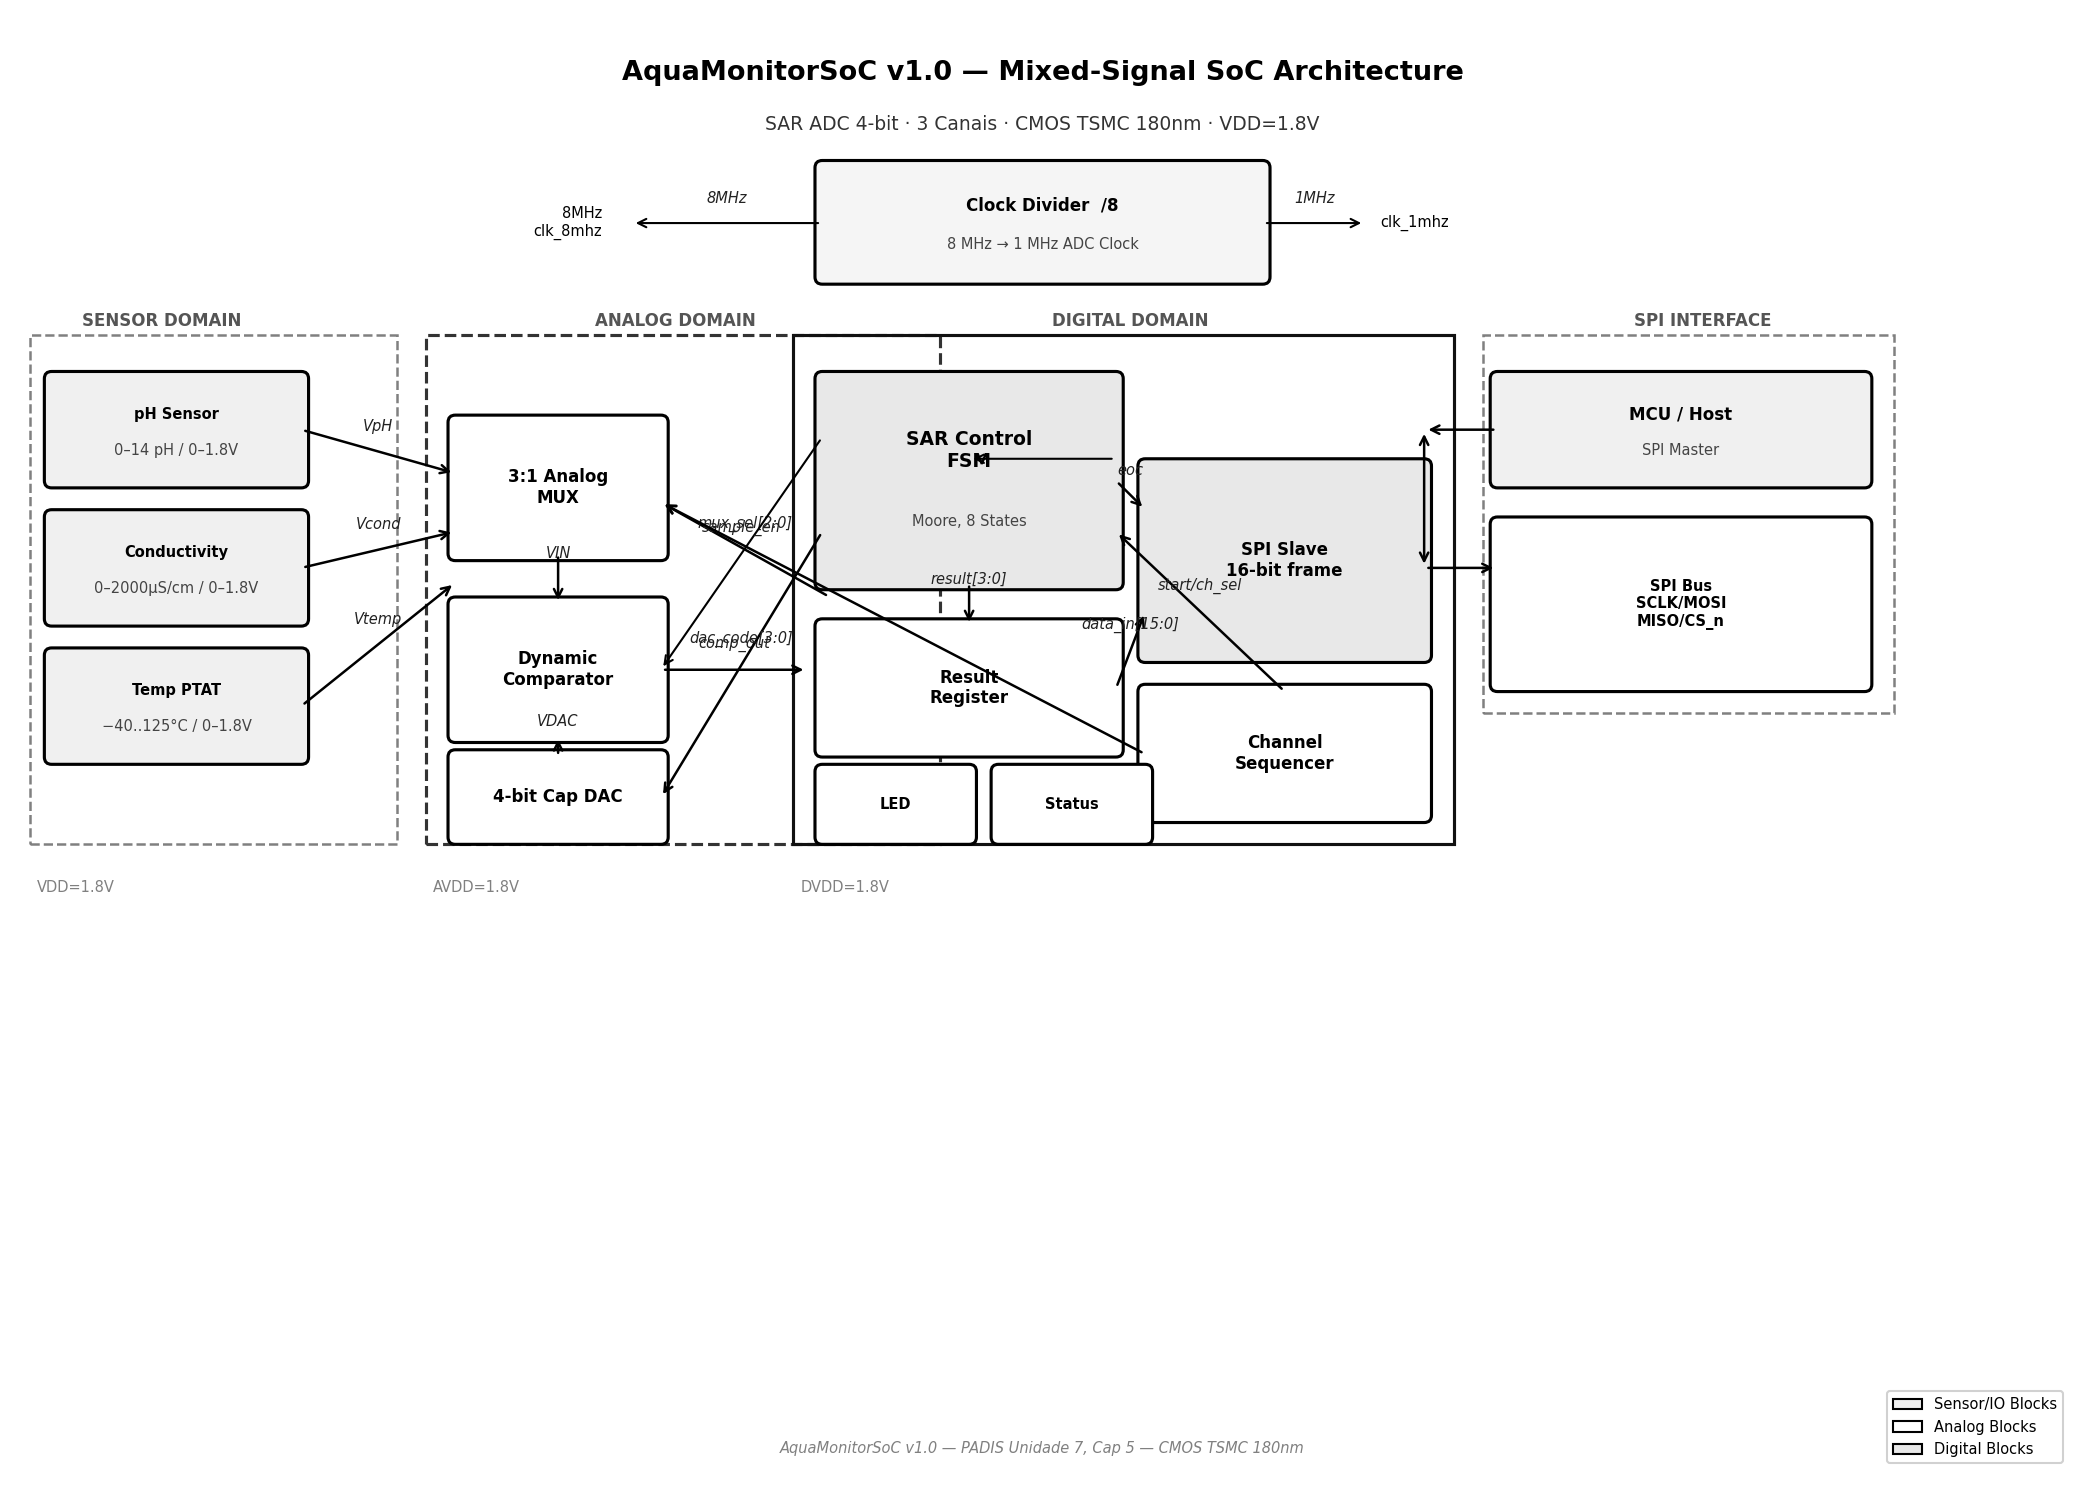
\includegraphics[width=\textwidth]{fig_arquitetura_soc.png}
  \caption{Arquitetura completa do AquaMonitorSoC v1.0. Blocos sensoriais (esquerda),
           domínio analógico interno (centro) e domínio digital (direita).}
  \label{fig:arq_soc}
\end{figure}

\subsection{Requisitos do Sistema}

\begin{specbox}{Especificação Geral do AquaMonitorSoC v1.0}
\begin{itemize}
  \item \textbf{Tecnologia:} CMOS TSMC 180nm, VDD = \SI{1.8}{\volt}
  \item \textbf{Clock:} Externo \SI{8}{\mega\hertz} $\to$ interno \SI{1}{\mega\hertz} via divisor /8
  \item \textbf{ADC:} SAR 4-bit, 1 conversor compartilhado (time-multiplexed)
  \item \textbf{Canais:} 3 (pH, Condutividade, Temperatura PTAT)
  \item \textbf{Latência por canal:} \SI{10}{\micro\second} (10 ciclos @ \SI{1}{\mega\hertz})
  \item \textbf{Latência total (3 canais):} \SI{30}{\micro\second}
  \item \textbf{Interface digital:} SPI escravo, quadro de 16 bits, CPOL=0, CPHA=0
  \item \textbf{Die estimado:} 800 $\times$ \SI{600}{\micro\meter}
\end{itemize}
\end{specbox}

\subsection{Especificação dos Canais Sensoriais}

\begin{table}[H]
  \centering
  \caption{Especificação dos canais sensoriais do AquaMonitorSoC v1.0}
  \label{tab:sensor_spec}
  \rowcolors{2}{bwlight}{white}
  \begin{tabularx}{\textwidth}{lXXXXX}
    \toprule
    \textbf{Parâmetro} & \textbf{Canal} & \textbf{Faixa Física} &
    \textbf{Faixa Elétrica} & \textbf{Resolução} & \textbf{Precisão} \\
    \midrule
    pH               & Ch0 & 0--14 pH        & 0--\SI{1.8}{\volt}  &
      0.875 pH (1 LSB) & $\pm$0.5 pH \\
    Condutividade    & Ch1 & 0--\SI{2000}{\micro\siemens\per\centi\meter} &
      0--\SI{1.8}{\volt} & \SI{125}{\micro\siemens\per\centi\meter} & $\pm$5\% \\
    Temperatura PTAT & Ch2 & --40 a \SI{125}{\celsius} & 0--\SI{1.8}{\volt} &
      \SI{10.3}{\celsius} (1 LSB) & $\pm$1$^\circ$C \\
    \bottomrule
  \end{tabularx}
\end{table}

\subsection{Especificação do ADC SAR}

\begin{table}[H]
  \centering
  \caption{Especificação do conversor SAR ADC 4-bit}
  \label{tab:adc_spec}
  \rowcolors{2}{bwlight}{white}
  \begin{tabular}{ll}
    \toprule
    \textbf{Parâmetro} & \textbf{Valor} \\
    \midrule
    Resolução           & 4 bits (16 níveis) \\
    Arquitetura         & Aproximação Sucessiva (SAR) \\
    Topologia do DAC    & Banco de capacitores ponderados binariamente \\
    Capacitor unitário  & $C_{unit} = \SI{20}{\femto\farad}$ \\
    Tensão de referência & \SI{1.8}{\volt} (VDD) \\
    LSB (tensão)        & $V_{LSB} = 1800/16 = \SI{112.5}{\milli\volt}$ \\
    Frequência de clock & \SI{1}{\mega\hertz} \\
    Ciclos por conversão & 10 (CH\_SEL + SAMPLE + 4$\times$BIT + DONE + idle) \\
    Taxa de conversão   & 100\,kSPS por canal \\
    Não-linearidade (INL) & < 0.5 LSB (estimativa) \\
    Não-linearidade (DNL) & < 0.5 LSB (estimativa) \\
    Consumo (analógico) & \textasciitilde{}\SI{150}{\micro\watt} \\
    \bottomrule
  \end{tabular}
\end{table}

\subsection{Especificação da Interface SPI}

\begin{table}[H]
  \centering
  \caption{Protocolo SPI do AquaMonitorSoC v1.0}
  \label{tab:spi_spec}
  \rowcolors{2}{bwlight}{white}
  \begin{tabular}{ll}
    \toprule
    \textbf{Parâmetro} & \textbf{Valor} \\
    \midrule
    Modo              & Escravo (SPI Slave) \\
    Polaridade/Fase   & CPOL=0, CPHA=0 (Modo 0) \\
    Tamanho do quadro & 16 bits \\
    Campo CH\_ID      & bits [15:12] — identificador do canal (4 bits) \\
    Campo RESULT      & bits [11:8]  — código ADC de 4 bits \\
    Campo STATUS      & bits [7:0]   — flags de estado \\
    STATUS[7]         & EOC — fim de conversão \\
    STATUS[6]         & OVERRUN — novo resultado antes de leitura \\
    STATUS[1:0]       & CH\_SEL\_ECHO — canal lido \\
    Velocidade máxima & \SI{4}{\mega\hertz} \\
    \bottomrule
  \end{tabular}
\end{table}

\newpage

% ============================================================
\section{Arquitetura do SoC}
\label{sec:arquitetura}
% ============================================================

\subsection{Particionamento Mixed-Signal}

A decisão fundamental no projeto de um SoC de sinal misto é o particionamento
entre os domínios analógico e digital. No AquaMonitorSoC v1.0, adotou-se a
separação física com fronteira nítida posicionada a 40\% da largura do die,
conforme ilustrado no floorplan da Figura~\ref{fig:floorplan}.

\textbf{Por que os blocos analógicos ficam à esquerda?}

\begin{enumerate}
  \item \textbf{Proximidade dos pads analógicos:} Os pads de entrada analógica
        (VpH, Vcond, Vtemp) são posicionados no lado esquerdo do die, minimizando
        o comprimento dos fios de metal que conduzem sinais de alta impedância e
        sensíveis a ruído;
  \item \textbf{Isolamento de substrato:} O ruído de chaveamento digital
        (dI/dt nas comutações CMOS) propaga-se pelo substrato. Ao posicionar
        os blocos analógicos longe dos blocos digitais e separados por anéis de
        guarda, reduz-se o acoplamento por substrato;
  \item \textbf{Roteamento de referências:} O bandgap de referência (\SI{1.2}{\volt})
        e a malha de terra analógico (AGND) ficam próximos dos circuitos que os
        utilizam (DAC, comparador), reduzindo resistência de fio e ruído de
        referência.
\end{enumerate}

\textbf{Por que os blocos digitais ficam à direita?}

\begin{enumerate}
  \item \textbf{Proximidade dos pads SPI:} Os pads SCLK, MOSI, MISO e CS\_n
        estão no lado direito, minimizando o comprimento das linhas de dados;
  \item \textbf{Centralização da distribuição de clock:} A árvore de clock
        digital (H-tree) é mais eficiente quando o bloco divisor de clock está
        próximo de todos os flip-flops digitais;
  \item \textbf{Área:} O domínio digital (SAR FSM + SPI + registradores) ocupa
        60\% da área útil, justificando sua posição central-direita.
\end{enumerate}

\begin{figure}[H]
  \centering
  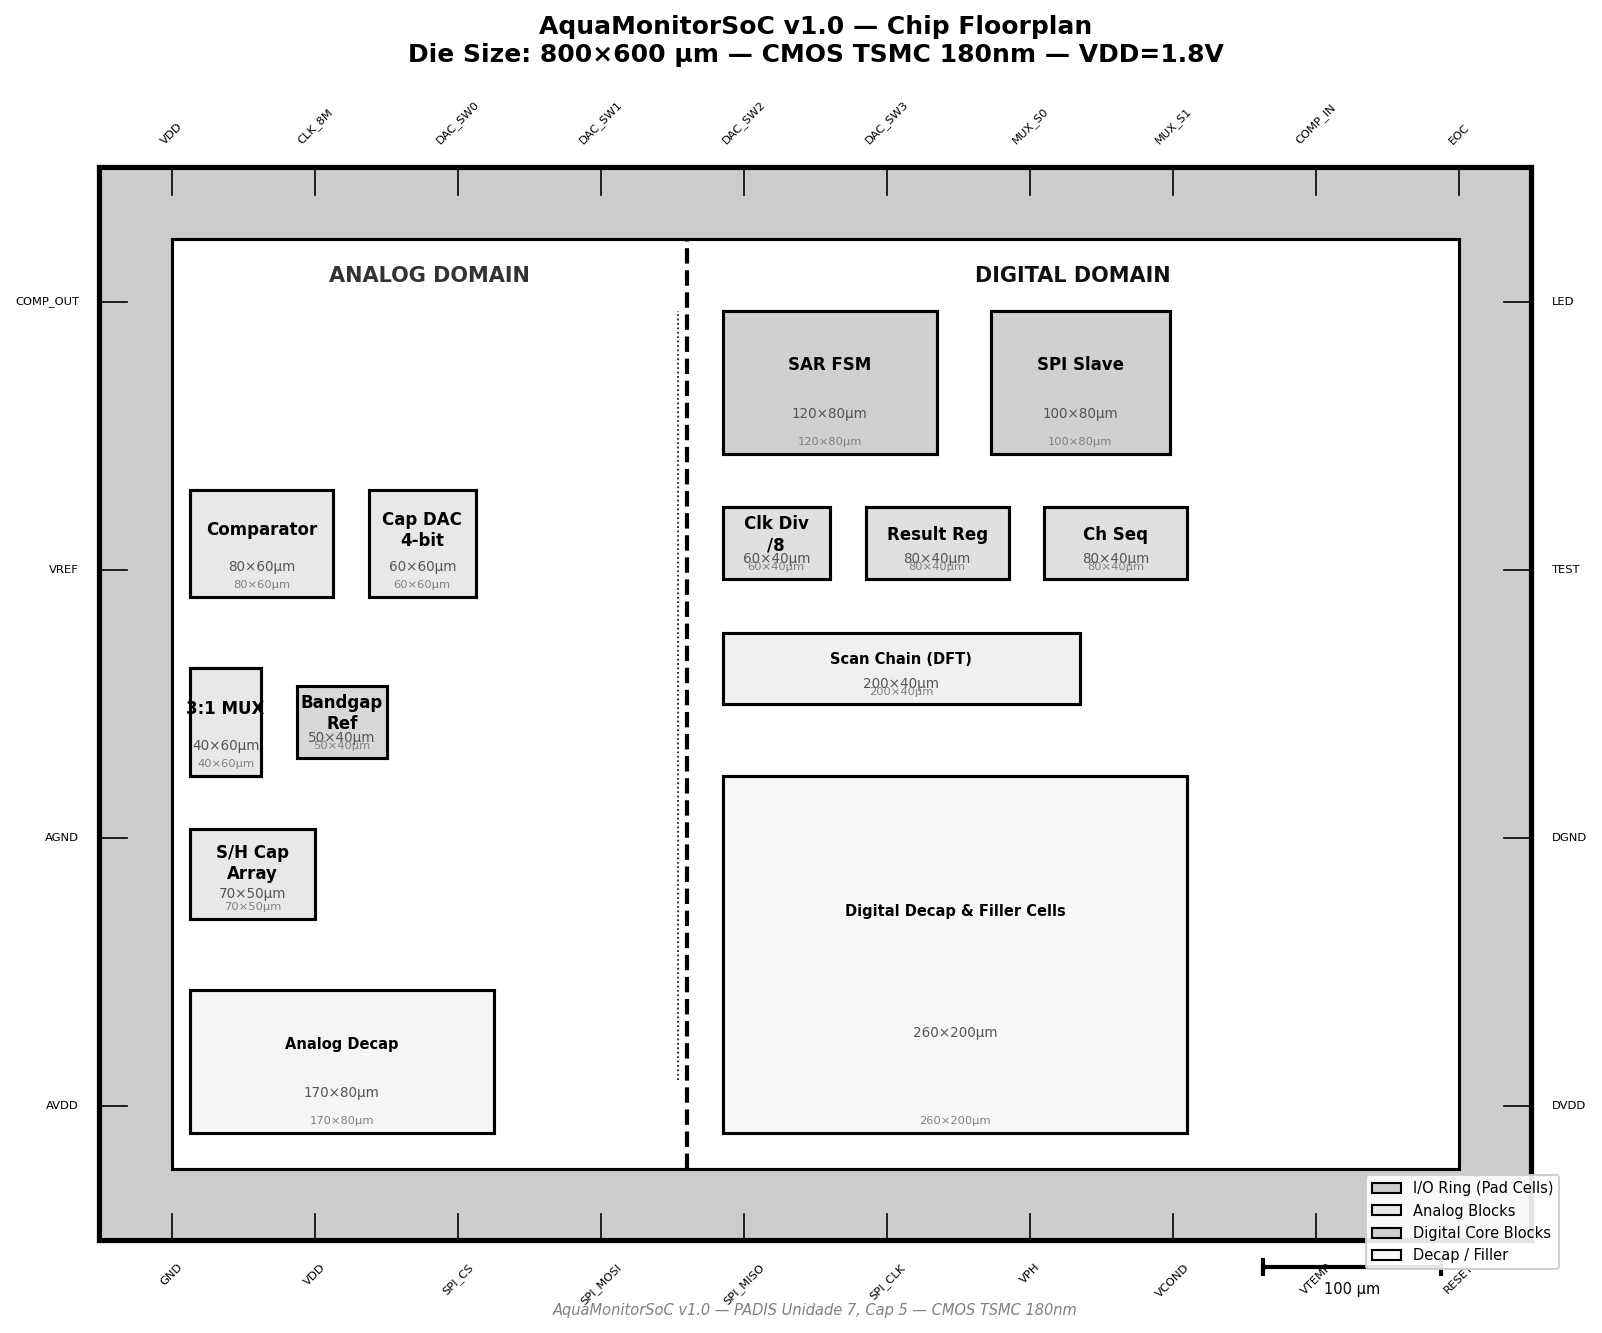
\includegraphics[width=\textwidth]{fig_floorplan_soc.png}
  \caption{Floorplan do AquaMonitorSoC v1.0. Die de 800$\times$\SI{600}{\micro\meter}
           com separação de domínios analógico (esq.) e digital (dir.).}
  \label{fig:floorplan}
\end{figure}

\subsection{Análise de Tradeoffs Arquiteturais}

A escolha da arquitetura de controle é o principal tradeoff deste projeto.
Três alternativas foram avaliadas: FSM dedicada (implementação atual),
núcleo RISC-V softcore e SoC externo ESP32.

\begin{figure}[H]
  \centering
  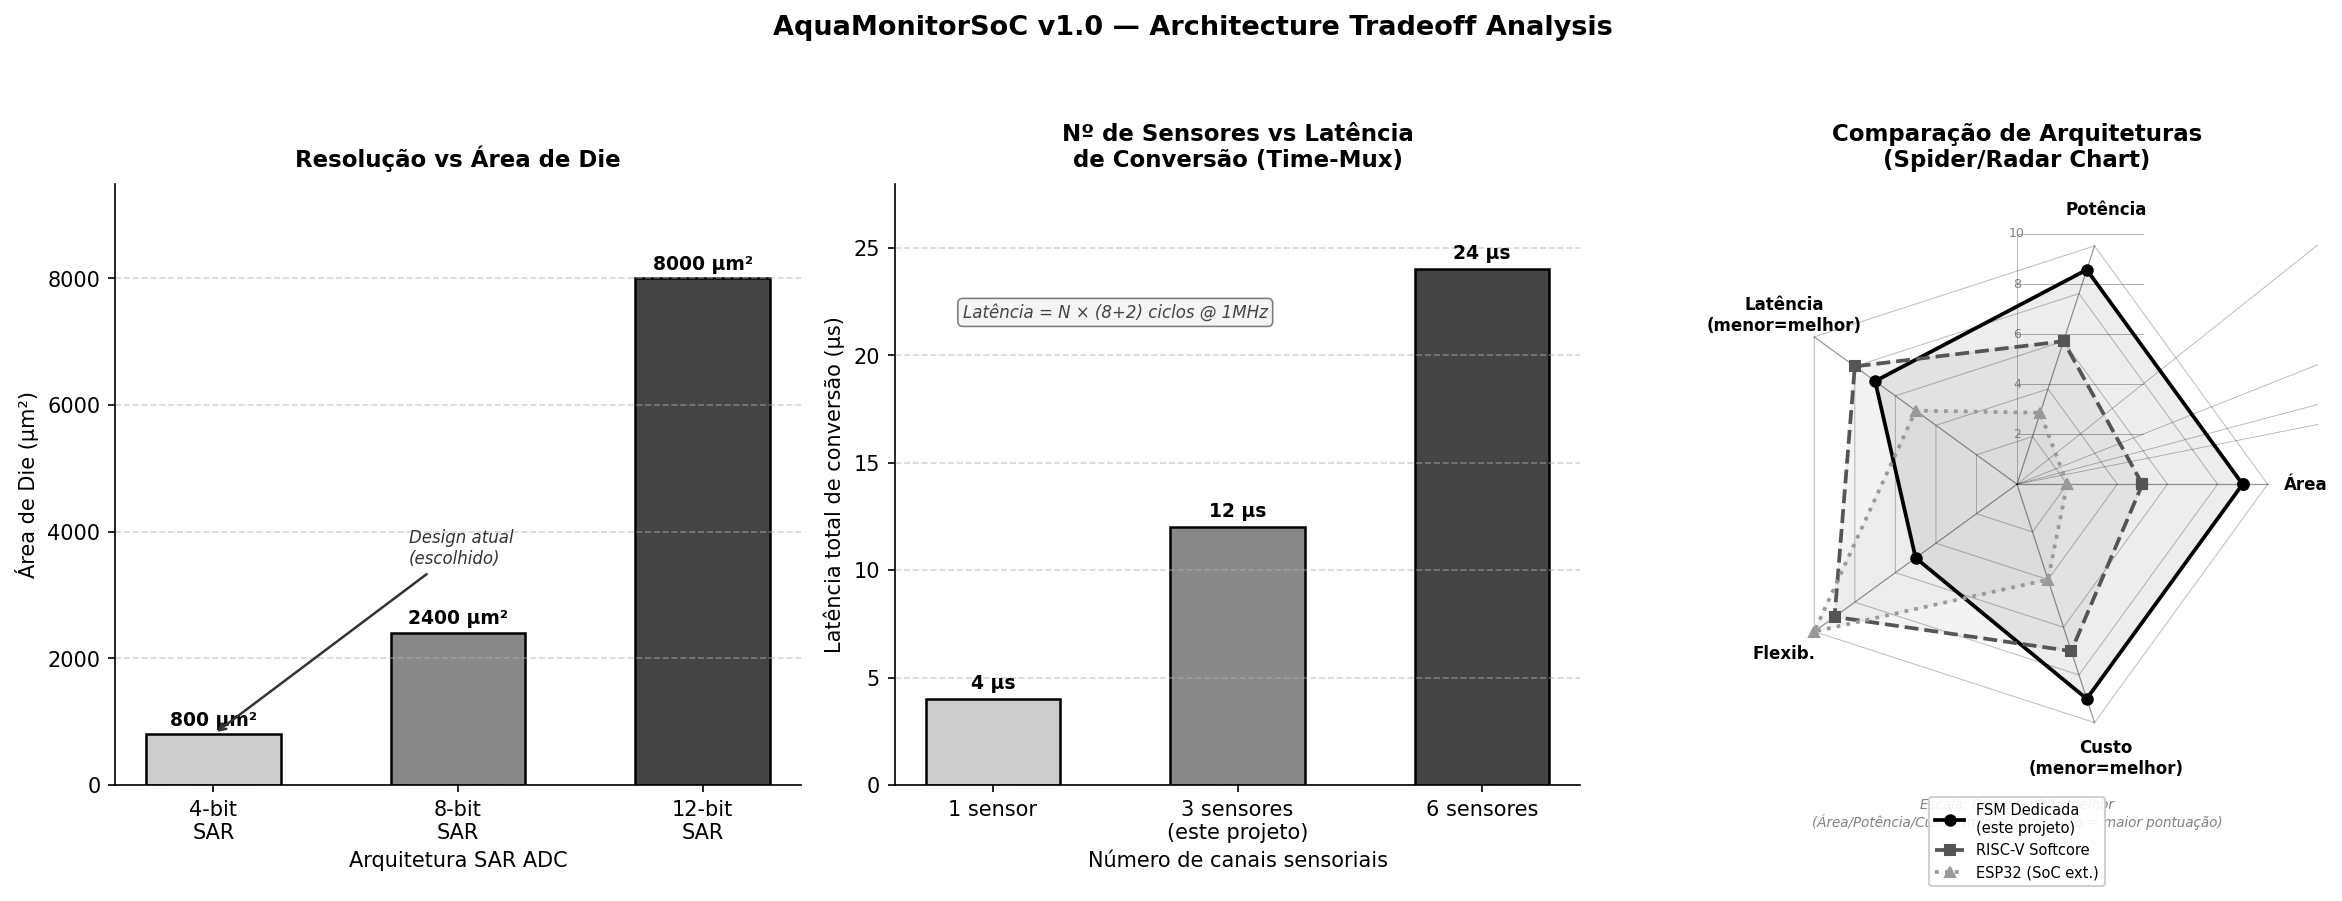
\includegraphics[width=\textwidth]{fig_tradeoffs.png}
  \caption{Análise de tradeoffs: resolução vs. área (esq.),
           latência vs. número de canais (centro),
           comparação de arquiteturas em radar (dir.).}
  \label{fig:tradeoffs}
\end{figure}

O Painel 1 da Figura~\ref{fig:tradeoffs} mostra que a área do DAC capacitivo
escala quadraticamente com a resolução: um SAR de 8 bits requer 3$\times$ mais área que
o de 4 bits ($\propto 2^N$ capacitores), enquanto o de 12 bits demanda 10$\times$.
Para a aplicação de piscicultura com 4 bits de resolução, a precisão é adequada
para pH ($\pm$0.875 pH, requisito $\leq$ $\pm$1 pH) e temperatura ($\pm$10$^\circ$C, compensável via
calibração).

O Painel 2 mostra que a latência total escala linearmente com o número de canais,
graças à multiplexação temporal. Para 6 sensores, a latência seria de
\SI{24}{\micro\second}, ainda compatível com amostragem a \SI{100}{\hertz}.

O Painel 3 (radar) sintetiza a comparação qualitativa: a FSM dedicada maximiza
eficiência em área e potência para esta aplicação específica; o RISC-V oferece
maior flexibilidade programática; o ESP32 tem máxima flexibilidade mas proibitivo
em potência para aplicações embarcadas sem fonte de alimentação contínua.

\subsection{Resumo de Área por Bloco}

\begin{table}[H]
  \centering
  \caption{Resumo de área estimada por bloco funcional}
  \label{tab:area_blocks}
  \rowcolors{2}{bwlight}{white}
  \begin{tabular}{llrr}
    \toprule
    \textbf{Bloco} & \textbf{Domínio} &
    \textbf{Dimensões ($\mu$m)} & \textbf{Área ($\mu$m$^2$)} \\
    \midrule
    Comparador dinâmico  & Analógico  & 80$\times$60  &  4\,800 \\
    DAC capacitivo 4-bit & Analógico  & 60$\times$60  &  3\,600 \\
    MUX analógico 3:1    & Analógico  & 40$\times$60  &  2\,400 \\
    Bandgap reference    & Analógico  & 50$\times$40  &  2\,000 \\
    S/H Cap Array        & Analógico  & 70$\times$50  &  3\,500 \\
    SAR FSM              & Digital    & 120$\times$80 &  9\,600 \\
    SPI Slave            & Digital    & 100$\times$80 &  8\,000 \\
    Divisor de clock /8  & Digital    & 60$\times$40  &  2\,400 \\
    Registrador resultado& Digital    & 80$\times$40  &  3\,200 \\
    Sequenciador canais  & Digital    & 80$\times$40  &  3\,200 \\
    Scan chain (DFT)     & Digital    & 200$\times$40 &  8\,000 \\
    Decap + filler       & Misto      & ---    & 42\,000 \\
    I/O ring (pads)      & I/O        & ---    & 57\,600 \\
    \midrule
    \textbf{Total die}   & ---        & 800$\times$600 & \textbf{480\,000} \\
    \bottomrule
  \end{tabular}
\end{table}

\newpage

% ============================================================
\section{Interface com Sensores}
\label{sec:sensors}
% ============================================================

\subsection{Circuitos de Condicionamento}

Cada canal sensor requer um circuito de condicionamento dedicado, responsável por
converter o sinal físico do transdutor para uma tensão compatível com o range de
entrada do ADC (0 a \SI{1.8}{\volt}), com baixa impedância de saída e proteção
contra sobretensão.

\begin{figure}[H]
  \centering
  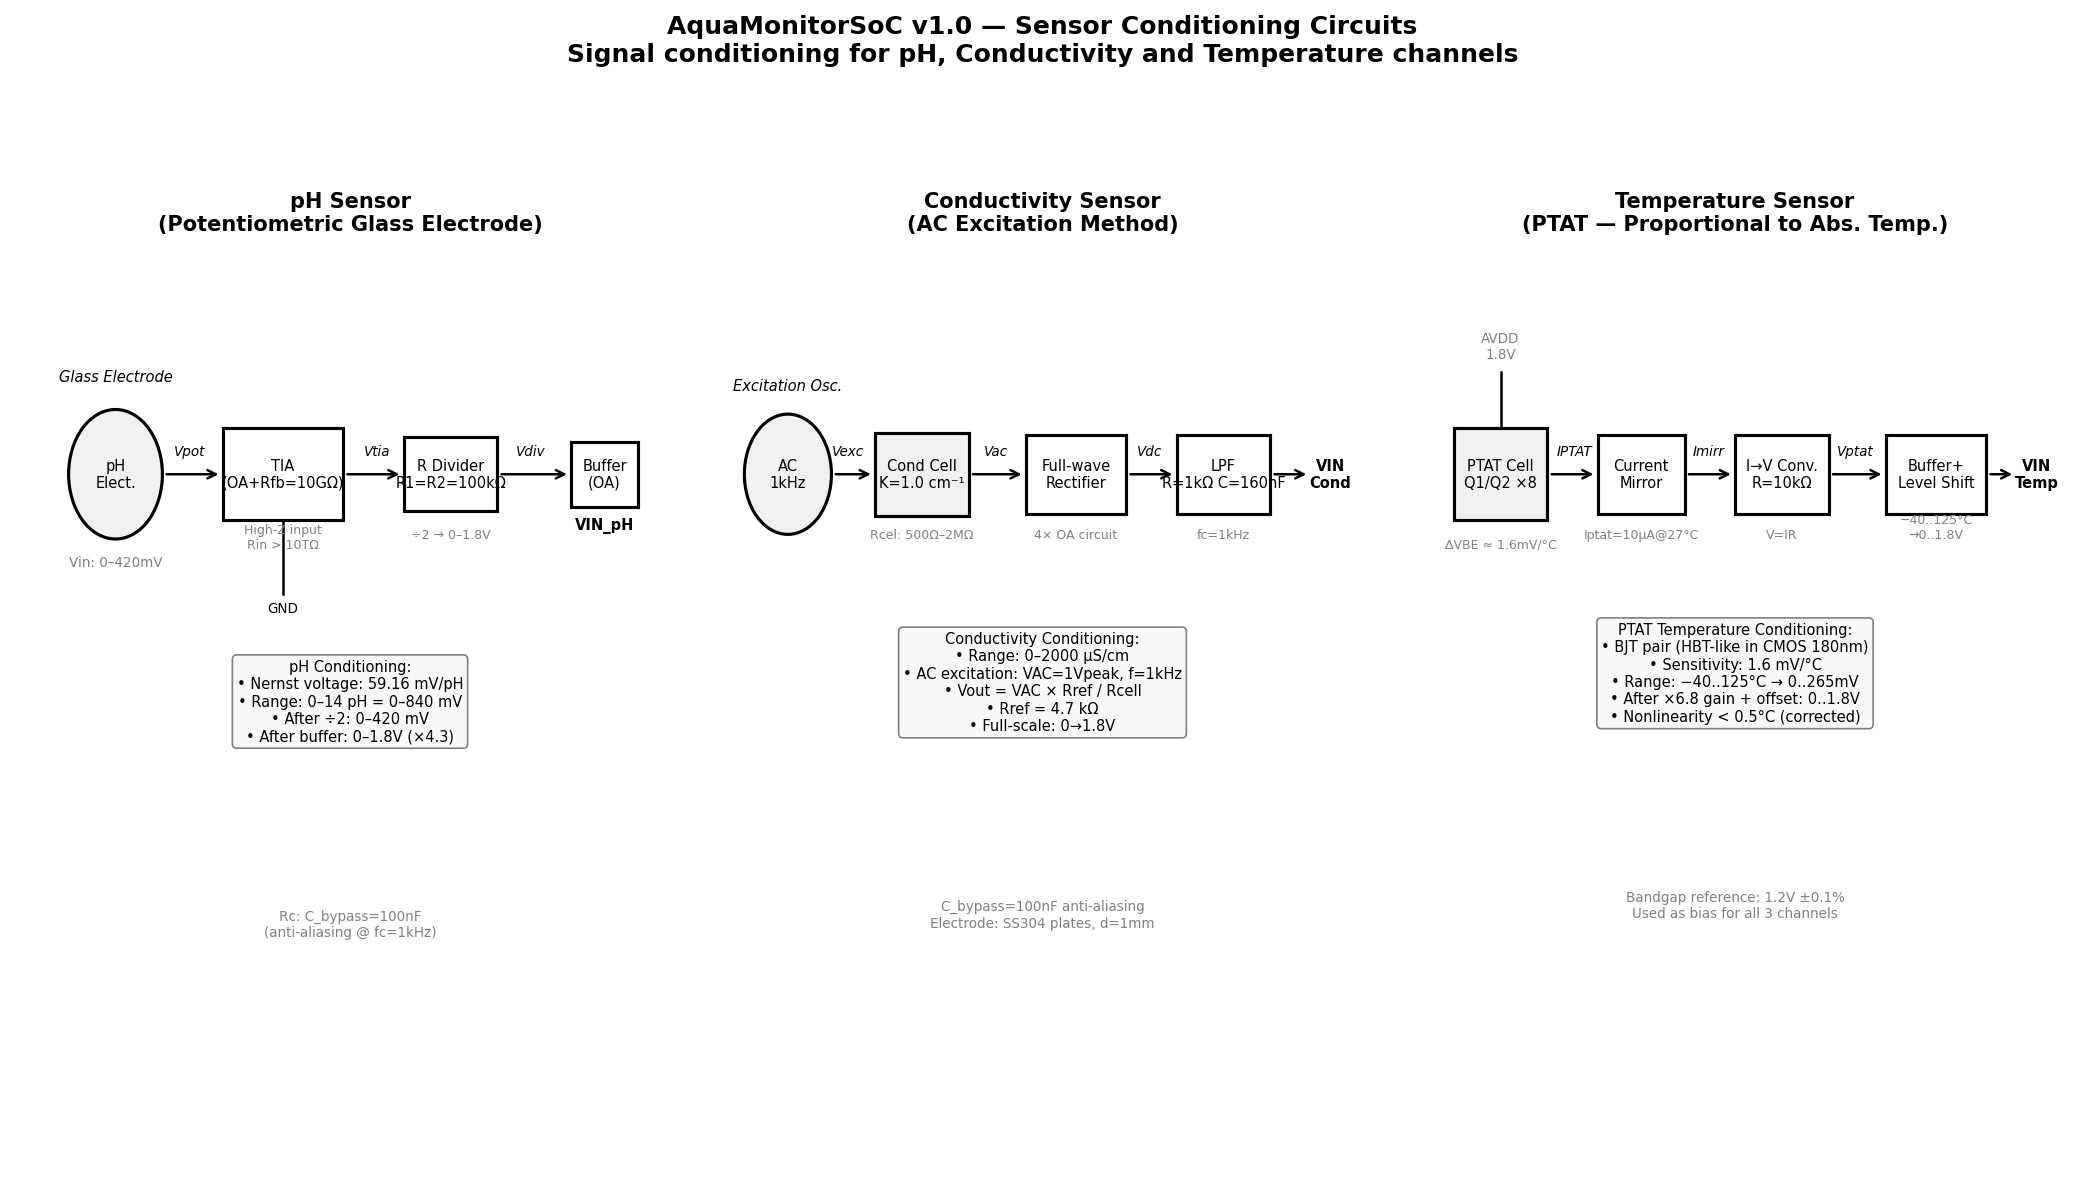
\includegraphics[width=\textwidth]{fig_sensor_interface.png}
  \caption{Circuitos de condicionamento dos três canais sensoriais:
           pH (esq.), condutividade (centro) e temperatura PTAT (dir.).}
  \label{fig:sensor_interface}
\end{figure}

\subsubsection{Canal de pH (Ch0)}

O eletrodo de vidro para pH gera uma tensão de Nernst de \SI{59.16}{\milli\volt}
por unidade de pH a \SI{25}{\celsius}, com impedância de saída tipicamente entre
\SI{100}{\mega\ohm} e \SI{1}{\giga\ohm}. O circuito de condicionamento utiliza:

\begin{enumerate}
  \item \textbf{Amplificador transimpedância (TIA):} OpAmp com realimentação
        $R_{fb} = \SI{10}{\giga\ohm}$ (resistor de proteção de eletrodo) e
        entrada de \textit{field-effect transistor} para altíssima impedância
        ($Z_{in} > \SI{10}{\tera\ohm}$);
  \item \textbf{Divisor resistivo:} $R_1 = R_2 = \SI{100}{\kilo\ohm}$, reduz a
        escala para compatibilidade com VDD = \SI{1.8}{\volt};
  \item \textbf{Buffer de saída:} OpAmp seguidor de tensão, $Z_{out} < \SI{1}{\ohm}$;
  \item \textbf{Capacitor anti-aliasing:} $C_{aa} = \SI{100}{\nano\farad}$,
        $f_c = \SI{1}{\kilo\hertz}$.
\end{enumerate}

\subsubsection{Canal de Condutividade (Ch1)}

A medição de condutividade utiliza excitação AC para evitar polarização
eletrolítica do eletrodo. O esquema emprega:

\begin{enumerate}
  \item \textbf{Oscilador de excitação:} \SI{1}{\kilo\hertz}, $V_{exc} = \SI{1}{\volt}_{pico}$;
  \item \textbf{Célula de condutividade:} Constante de célula $K = \SI{1.0}{\per\centi\meter}$,
        resistência $R_{cel} = K/G$ onde $G$ é a condutância medida;
  \item \textbf{Retificador de onda completa:} Baseado em 4 OpAmps, retifica o
        sinal AC para tensão DC proporcional à amplitude;
  \item \textbf{Filtro passa-baixa:} $R = \SI{1}{\kilo\ohm}$, $C = \SI{160}{\nano\farad}$,
        $f_c = \SI{1}{\kilo\hertz}$, remove o ripple da excitação.
\end{enumerate}

\subsubsection{Canal de Temperatura PTAT (Ch2)}

A célula de temperatura utiliza a propriedade Proporcional à Temperatura Absoluta
(PTAT) de junctions PN bipolares em CMOS 180nm:

\begin{enumerate}
  \item \textbf{Par de BJTs:} $Q_1$ e $Q_2$ com razão de área $r = 8$;
        $\Delta V_{BE} = V_T \ln(r) \approx \SI{1.6}{\milli\volt\per\celsius}$;
  \item \textbf{Espelho de corrente PTAT:} $I_{PTAT} = \SI{10}{\micro\ampere}$
        a \SI{27}{\celsius};
  \item \textbf{Conversor I$\to$V:} $R_{conv} = \SI{10}{\kilo\ohm}$;
  \item \textbf{Buffer + Deslocamento de nível:} Ajusta a faixa --40 a \SI{125}{\celsius}
        para 0 a \SI{1.8}{\volt} com amplificação $A_v = 6.8$ e offset de \SI{-400}{\milli\volt}.
\end{enumerate}

\subsection{Tabela de Atribuição de Pinos}

\begin{table}[H]
  \centering
  \caption{Atribuição de pinos do AquaMonitorSoC v1.0}
  \label{tab:pinout}
  \rowcolors{2}{bwlight}{white}
  \begin{tabular}{llll}
    \toprule
    \textbf{Pino} & \textbf{Direção} & \textbf{Tipo} & \textbf{Descrição} \\
    \midrule
    VPH       & Input  & Analógico & Entrada pH (0--\SI{1.8}{\volt}) \\
    VCOND     & Input  & Analógico & Entrada condutividade \\
    VTEMP     & Input  & Analógico & Entrada temperatura PTAT \\
    COMP\_IN  & Input  & Analógico & Entrada comparador dinâmico \\
    COMP\_OUT & Output & Analógico & Saída comparador (para FSM) \\
    DAC\_SW[3:0] & Output & Digital & Chaves do DAC capacitivo \\
    MUX\_S[2:0]  & Output & Digital & Seleção MUX analógico \\
    SPI\_CS   & Input  & Digital   & Chip Select SPI (ativo baixo) \\
    SPI\_MOSI & Input  & Digital   & Dados SPI entrada \\
    SPI\_MISO & Output & Digital   & Dados SPI saída \\
    SPI\_CLK  & Input  & Digital   & Clock SPI \\
    CLK\_8M   & Input  & Digital   & Clock externo \SI{8}{\mega\hertz} \\
    RESET     & Input  & Digital   & Reset assíncrono ativo baixo \\
    EOC       & Output & Digital   & Fim de conversão (pulso) \\
    LED       & Output & Digital   & Indicador status \\
    VDD / GND & ---    & Alimentação & \SI{1.8}{\volt} / Terra \\
    AVDD / AGND & ---  & Alimentação & Analógico \SI{1.8}{\volt} / Terra \\
    \bottomrule
  \end{tabular}
\end{table}

\newpage

% ============================================================
\section{Design Analógico  --  SAR ADC}
\label{sec:analog}
% ============================================================

\subsection{Comparador Dinâmico}

O comparador dinâmico é o bloco analógico mais crítico do SAR ADC. Reutilizando
o projeto desenvolvido nas unidades anteriores do PADIS, o comparador emprega
uma topologia StrongARM \textit{latch} com regeneração positiva, projetada
especificamente em CMOS 180nm com VDD = \SI{1.8}{\volt}.

\begin{figure}[H]
  \centering
  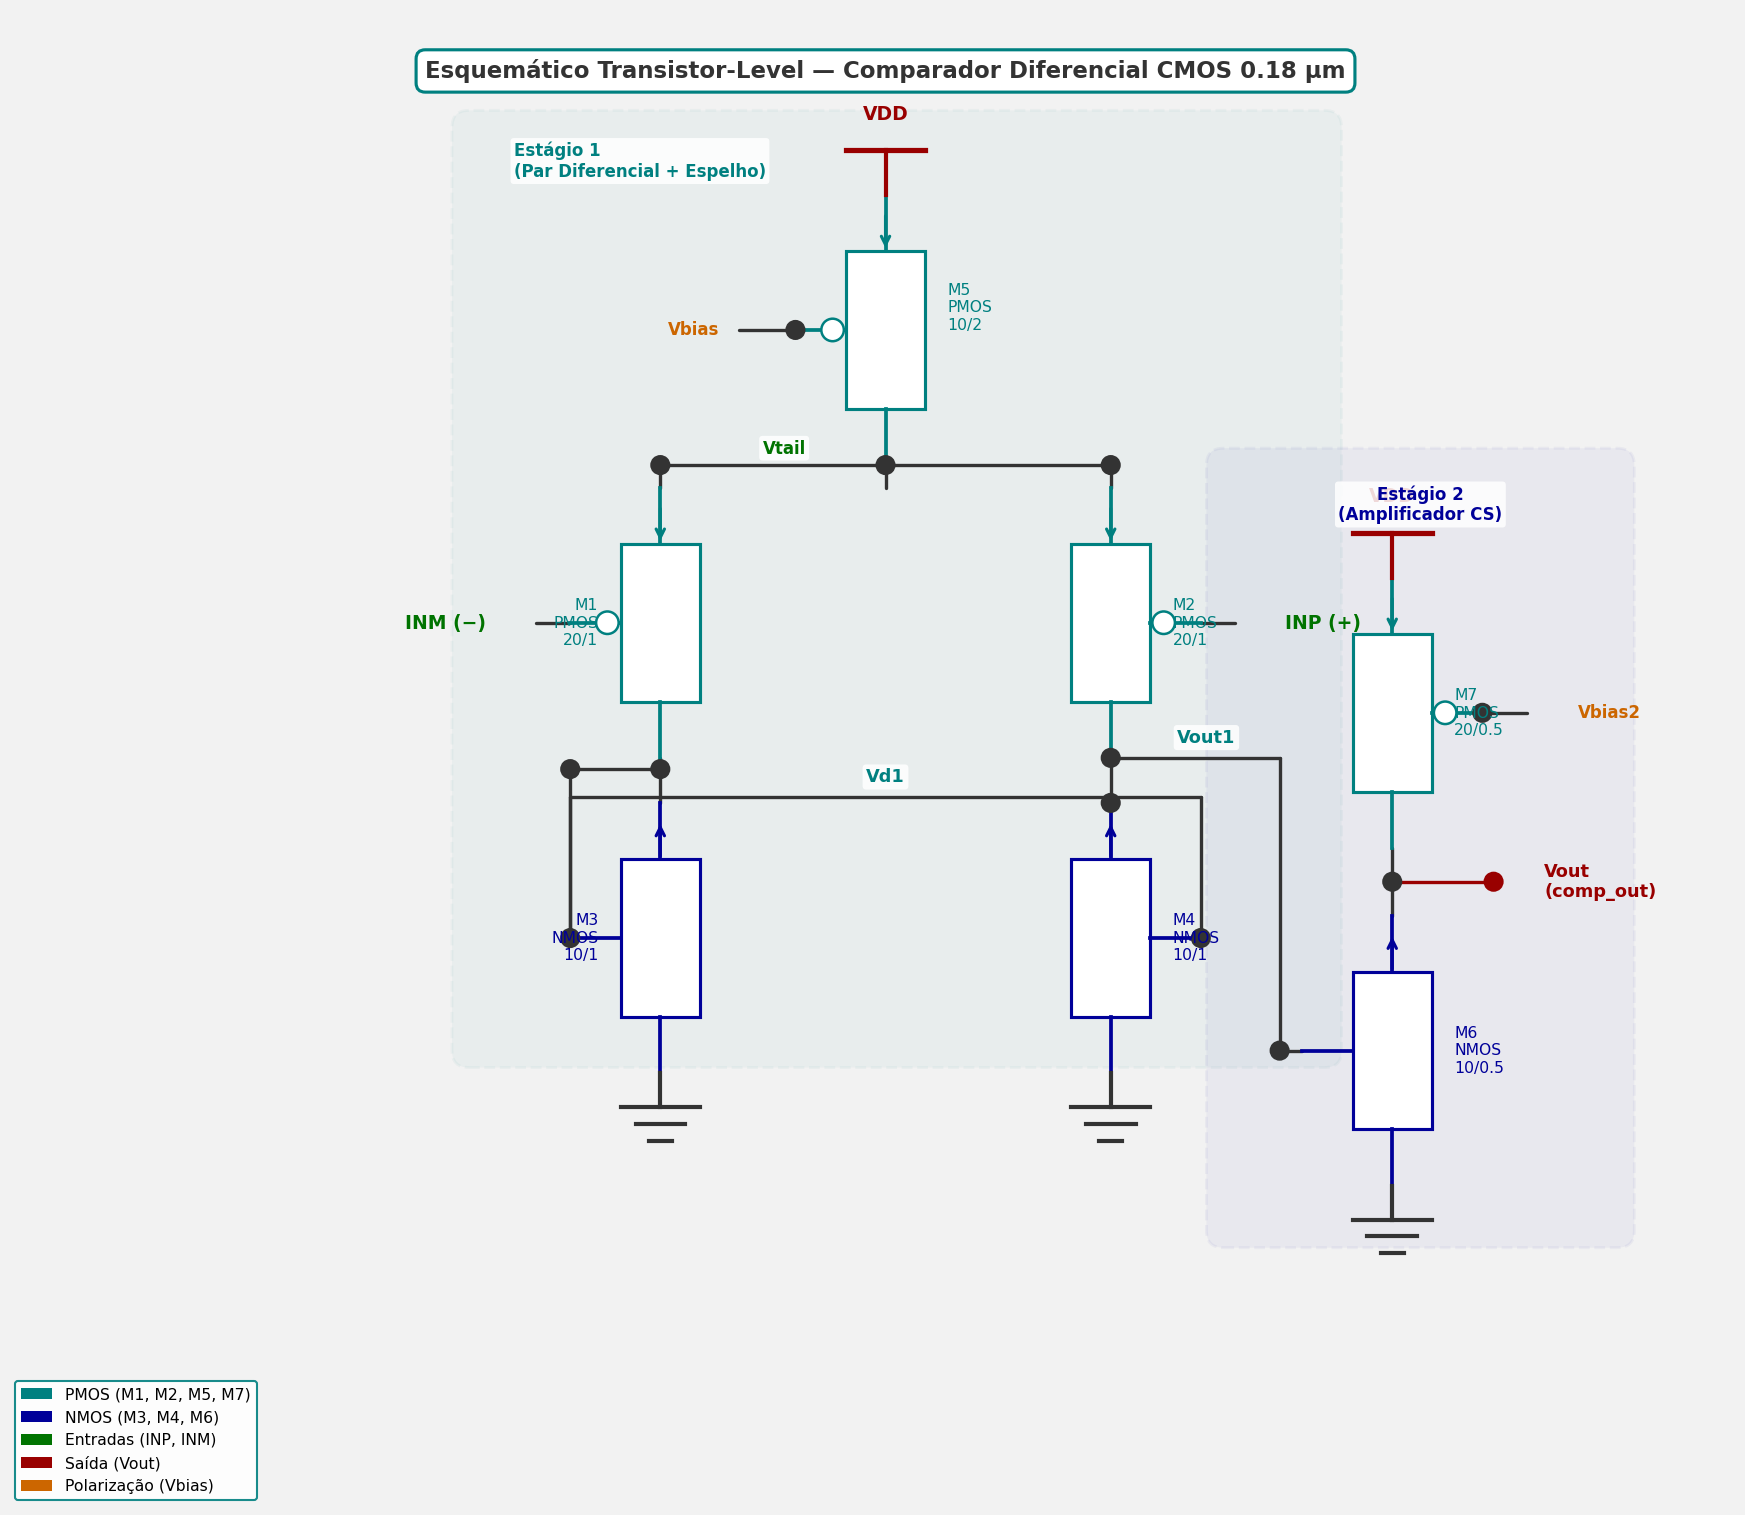
\includegraphics[width=0.48\textwidth]{../microeletronica/fig_schem_comparator.png}
  \hspace{0.02\textwidth}
  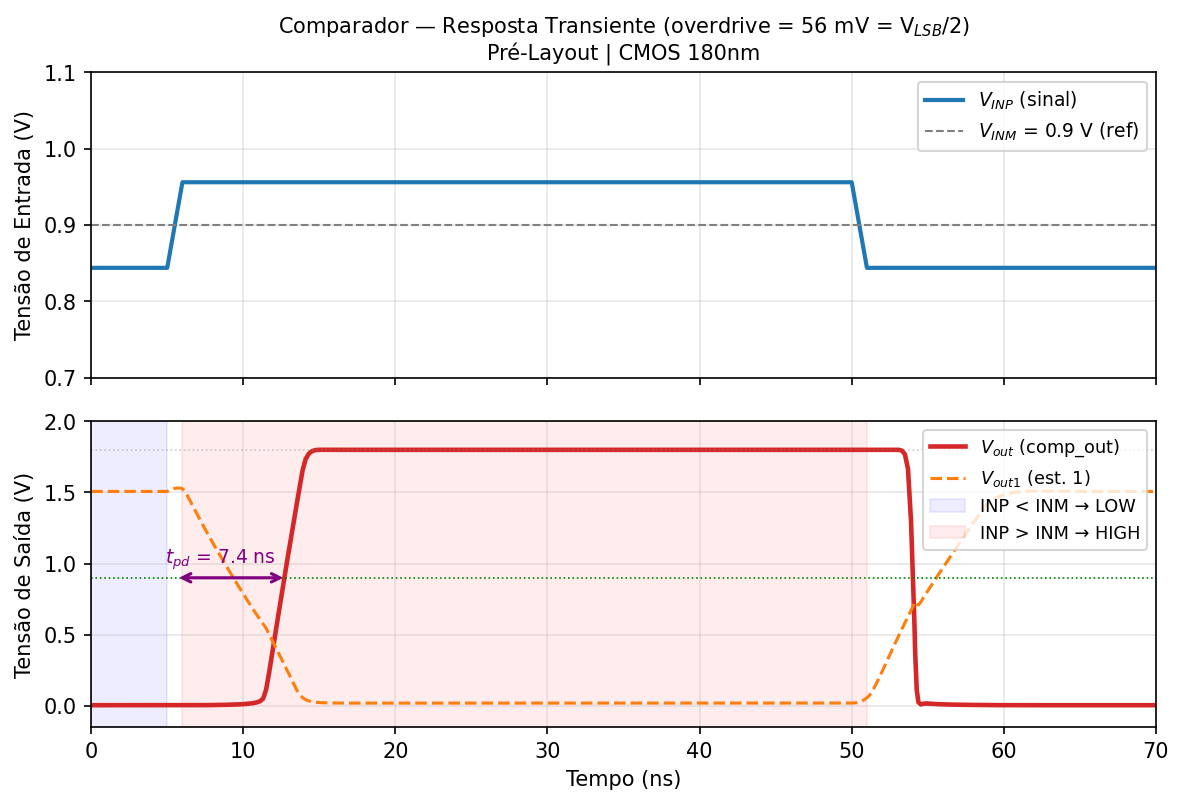
\includegraphics[width=0.46\textwidth]{../microeletronica/fig_comp_transiente.png}
  \caption{Esquerda: esquemático do comparador dinâmico (CMOS 180nm).
           Direita: resposta transiente  --  saída latch em função de $\Delta V_{in}$.}
  \label{fig:comparador}
\end{figure}

As principais especificações do comparador são:

\begin{table}[H]
  \centering
  \caption{Especificações do comparador dinâmico}
  \label{tab:comp_spec}
  \rowcolors{2}{bwlight}{white}
  \begin{tabular}{ll}
    \toprule
    \textbf{Parâmetro} & \textbf{Valor} \\
    \midrule
    Topologia             & StrongARM latch \\
    Tensão de offset (TT, 27$^\circ$C) & $V_{os} < \SI{5}{\milli\volt}$ \\
    Tensão de offset (pior canto) & $V_{os} < \SI{15}{\milli\volt}$ \\
    Tempo de regeneração  & $\tau_{regen} < \SI{200}{\nano\second}$ \\
    Tensão de entrada mínima & $\Delta V_{in,min} = V_{LSB}/2 = \SI{56.25}{\milli\volt}$ \\
    Consumo (energia/decisão) & \SI{50}{\femto\joule} \\
    \bottomrule
  \end{tabular}
\end{table}

\subsection{DAC Capacitivo de 4 Bits}

O DAC capacitivo é implementado como um banco de capacitores ponderados
binariamente (\textit{binary-weighted capacitor array}):

\begin{equation}
  V_{DAC} = V_{ref} \cdot \frac{\sum_{i=0}^{3} b_i \cdot 2^i \cdot C_{unit}}{C_{total}}
  = V_{ref} \cdot \frac{D}{16}
\end{equation}

\noindent onde $D$ é o código digital de 4 bits, $C_{unit} = \SI{20}{\femto\farad}$
e $V_{ref} = V_{DD} = \SI{1.8}{\volt}$.

\begin{table}[H]
  \centering
  \caption{Dimensionamento dos capacitores do DAC}
  \label{tab:dac_caps}
  \rowcolors{2}{bwlight}{white}
  \begin{tabular}{llll}
    \toprule
    \textbf{Bit} & \textbf{Peso} & \textbf{Capacitância} & \textbf{Área estimada ($\mu$m$^2$)} \\
    \midrule
    $b_3$ (MSB) & $8 \times C_{unit}$ & \SI{160}{\femto\farad} & 64 \\
    $b_2$       & $4 \times C_{unit}$ & \SI{80}{\femto\farad}  & 32 \\
    $b_1$       & $2 \times C_{unit}$ & \SI{40}{\femto\farad}  & 16 \\
    $b_0$ (LSB) & $1 \times C_{unit}$ & \SI{20}{\femto\farad}  & 8  \\
    $C_{term}$  & $1 \times C_{unit}$ & \SI{20}{\femto\farad}  & 8  \\
    \midrule
    \textbf{Total} & $16 \times C_{unit}$ & \SI{320}{\femto\farad} & \textbf{128} \\
    \bottomrule
  \end{tabular}
\end{table}

\subsection{Análise de Ruído}

O ruído térmico na amostragem do capacitor S/H impõe um limite fundamental
de resolução dado pela relação kT/C:

\begin{equation}
  V_{n,rms} = \sqrt{\frac{kT}{C_{sample}}} = \sqrt{\frac{1.38 \times 10^{-23} \times 300}{320 \times 10^{-15}}} \approx \SI{3.6}{\micro\volt}
\end{equation}

Para um ADC de 4 bits, o LSB é \SI{112.5}{\milli\volt} e a tensão de ruído
equivalente de quantização é $V_{q,rms} = LSB/\sqrt{12} \approx \SI{32.5}{\milli\volt}$.
Como $V_{n,rms} \ll V_{q,rms}$, o ruído kT/C é desprezível e não limita a
resolução de 4 bits. Mesmo para 8 bits ($LSB = \SI{7}{\milli\volt}$, $V_{q,rms} = \SI{2}{\milli\volt}$),
o ruído kT/C ainda seria inferior ao ruído de quantização.

\subsection{Especificação de Offset do Comparador}

O offset do comparador introduz um erro sistemático nas conversões SAR. Para que
o erro seja inferior a 0.5 LSB:

\begin{equation}
  |V_{os}| < \frac{V_{LSB}}{2} = \frac{\SI{112.5}{\milli\volt}}{2} = \SI{56.25}{\milli\volt}
\end{equation}

O comparador projetado em CMOS 180nm apresenta $|V_{os}| < \SI{5}{\milli\volt}$
no canto TT/27$^\circ$C, com variação de até \SI{15}{\milli\volt} nos cantos extremos,
permanecendo dentro da especificação em todos os casos.

\newpage

% ============================================================
\section{Design Digital  --  FSM de Controle SAR}
\label{sec:fsm}
% ============================================================

\subsection{Descrição dos Estados}

A FSM de controle SAR é implementada como uma máquina de Moore com 8 estados,
onde as saídas dependem exclusivamente do estado atual (não das entradas).
A Figura~\ref{fig:fsm} apresenta o diagrama de estados completo.

\begin{figure}[H]
  \centering
  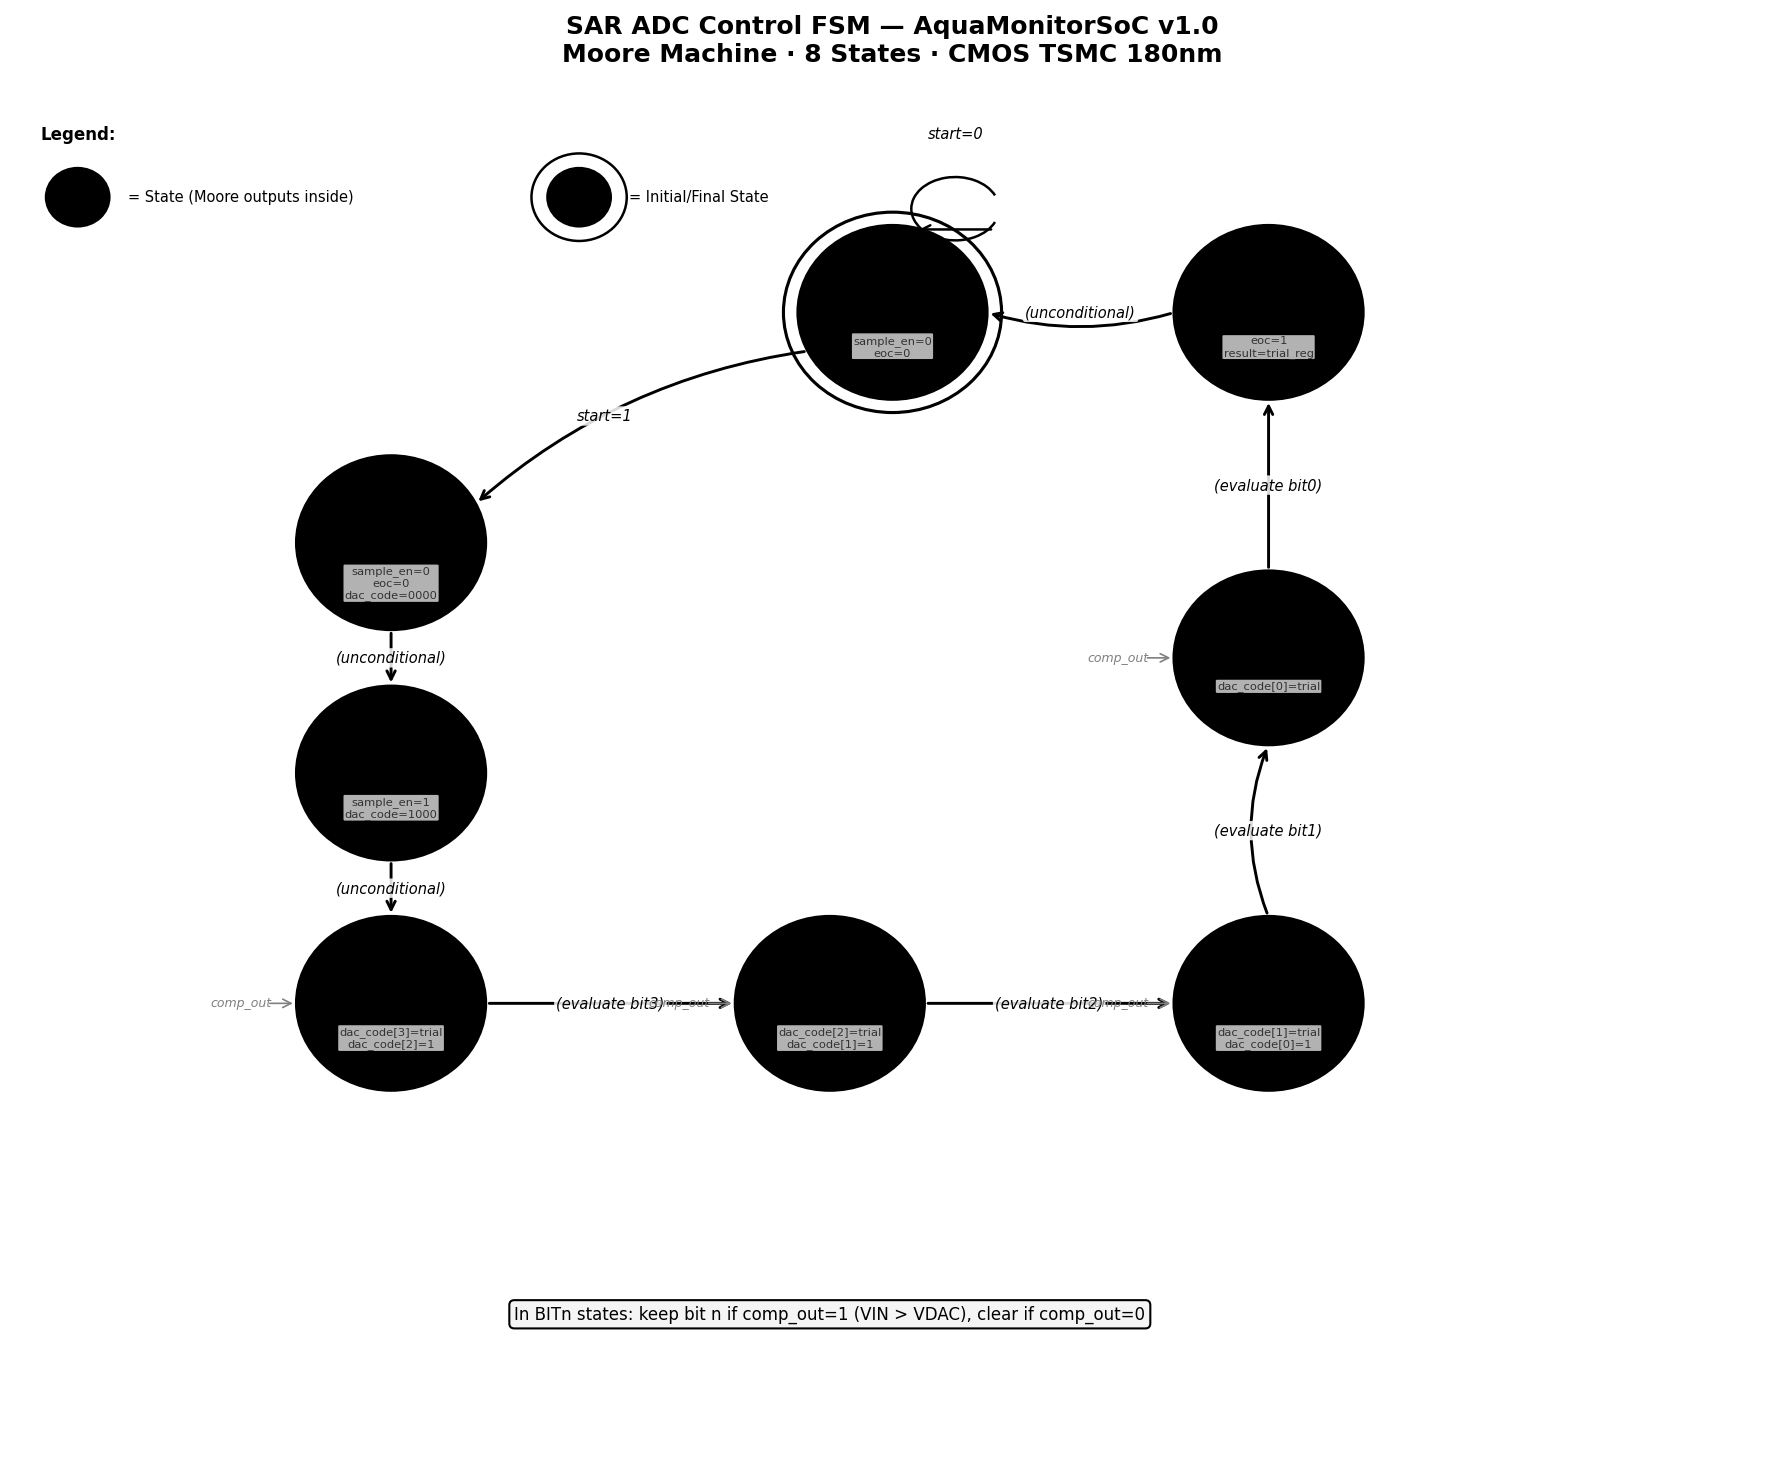
\includegraphics[width=\textwidth]{fig_fsm_states.png}
  \caption{Diagrama de estados da FSM SAR  --  8 estados Moore.
           As saídas de cada estado estão indicadas dentro dos círculos.}
  \label{fig:fsm}
\end{figure}

\begin{table}[H]
  \centering
  \caption{Tabela de estados da FSM SAR}
  \label{tab:state_table}
  \rowcolors{2}{bwlight}{white}
  \begin{tabular}{lllll}
    \toprule
    \textbf{Estado} & \textbf{Código} & \textbf{sample\_en} &
    \textbf{eoc} & \textbf{dac\_code} \\
    \midrule
    IDLE   & 4'h0 & 0 & 0 & trial\_reg (mantém) \\
    CH\_SEL & 4'h1 & 0 & 0 & 4'b0000 (limpa) \\
    SAMPLE & 4'h2 & 1 & 0 & 4'b1000 (MSB trial) \\
    BIT3   & 4'h3 & 0 & 0 & trial\_reg (avaliar b3) \\
    BIT2   & 4'h4 & 0 & 0 & trial\_reg (avaliar b2) \\
    BIT1   & 4'h5 & 0 & 0 & trial\_reg (avaliar b1) \\
    BIT0   & 4'h6 & 0 & 0 & trial\_reg (avaliar b0) \\
    DONE   & 4'h7 & 0 & 1 & trial\_reg (resultado) \\
    \bottomrule
  \end{tabular}
\end{table}

\subsection{Algoritmo SAR}

O algoritmo de aproximação sucessiva opera bit a bit do MSB ao LSB:

\begin{enumerate}
  \item \textbf{IDLE:} Aguarda o sinal \texttt{start} do sequenciador de canais;
  \item \textbf{CH\_SEL:} Seleciona o canal analógico; limpa o registrador \texttt{trial\_reg};
  \item \textbf{SAMPLE:} Ativa \texttt{sample\_en} para carregar o capacitor S/H
        com a tensão do canal selecionado; define DAC = 4'b1000 (8/16 da referência);
  \item \textbf{BIT3--BIT0:} Em cada estado BITn:
    \begin{itemize}
      \item O DAC apresenta \texttt{trial\_reg} ao comparador;
      \item Na próxima borda de clock, se \texttt{comparator\_out=1} (VIN > VDAC),
            o bit $n$ é \textbf{mantido} em 1 (VIN é maior, o bit é verdadeiro);
      \item Se \texttt{comparator\_out=0}, o bit $n$ é \textbf{limpo} para 0;
      \item O próximo bit ($n-1$) é tentado em 1;
    \end{itemize}
  \item \textbf{DONE:} Pulsa \texttt{eoc=1} por um ciclo; latch do resultado
        em \texttt{result[3:0]};
  \item Retorna a \textbf{IDLE}.
\end{enumerate}

\subsection{Análise de Timing}

\begin{figure}[H]
  \centering
  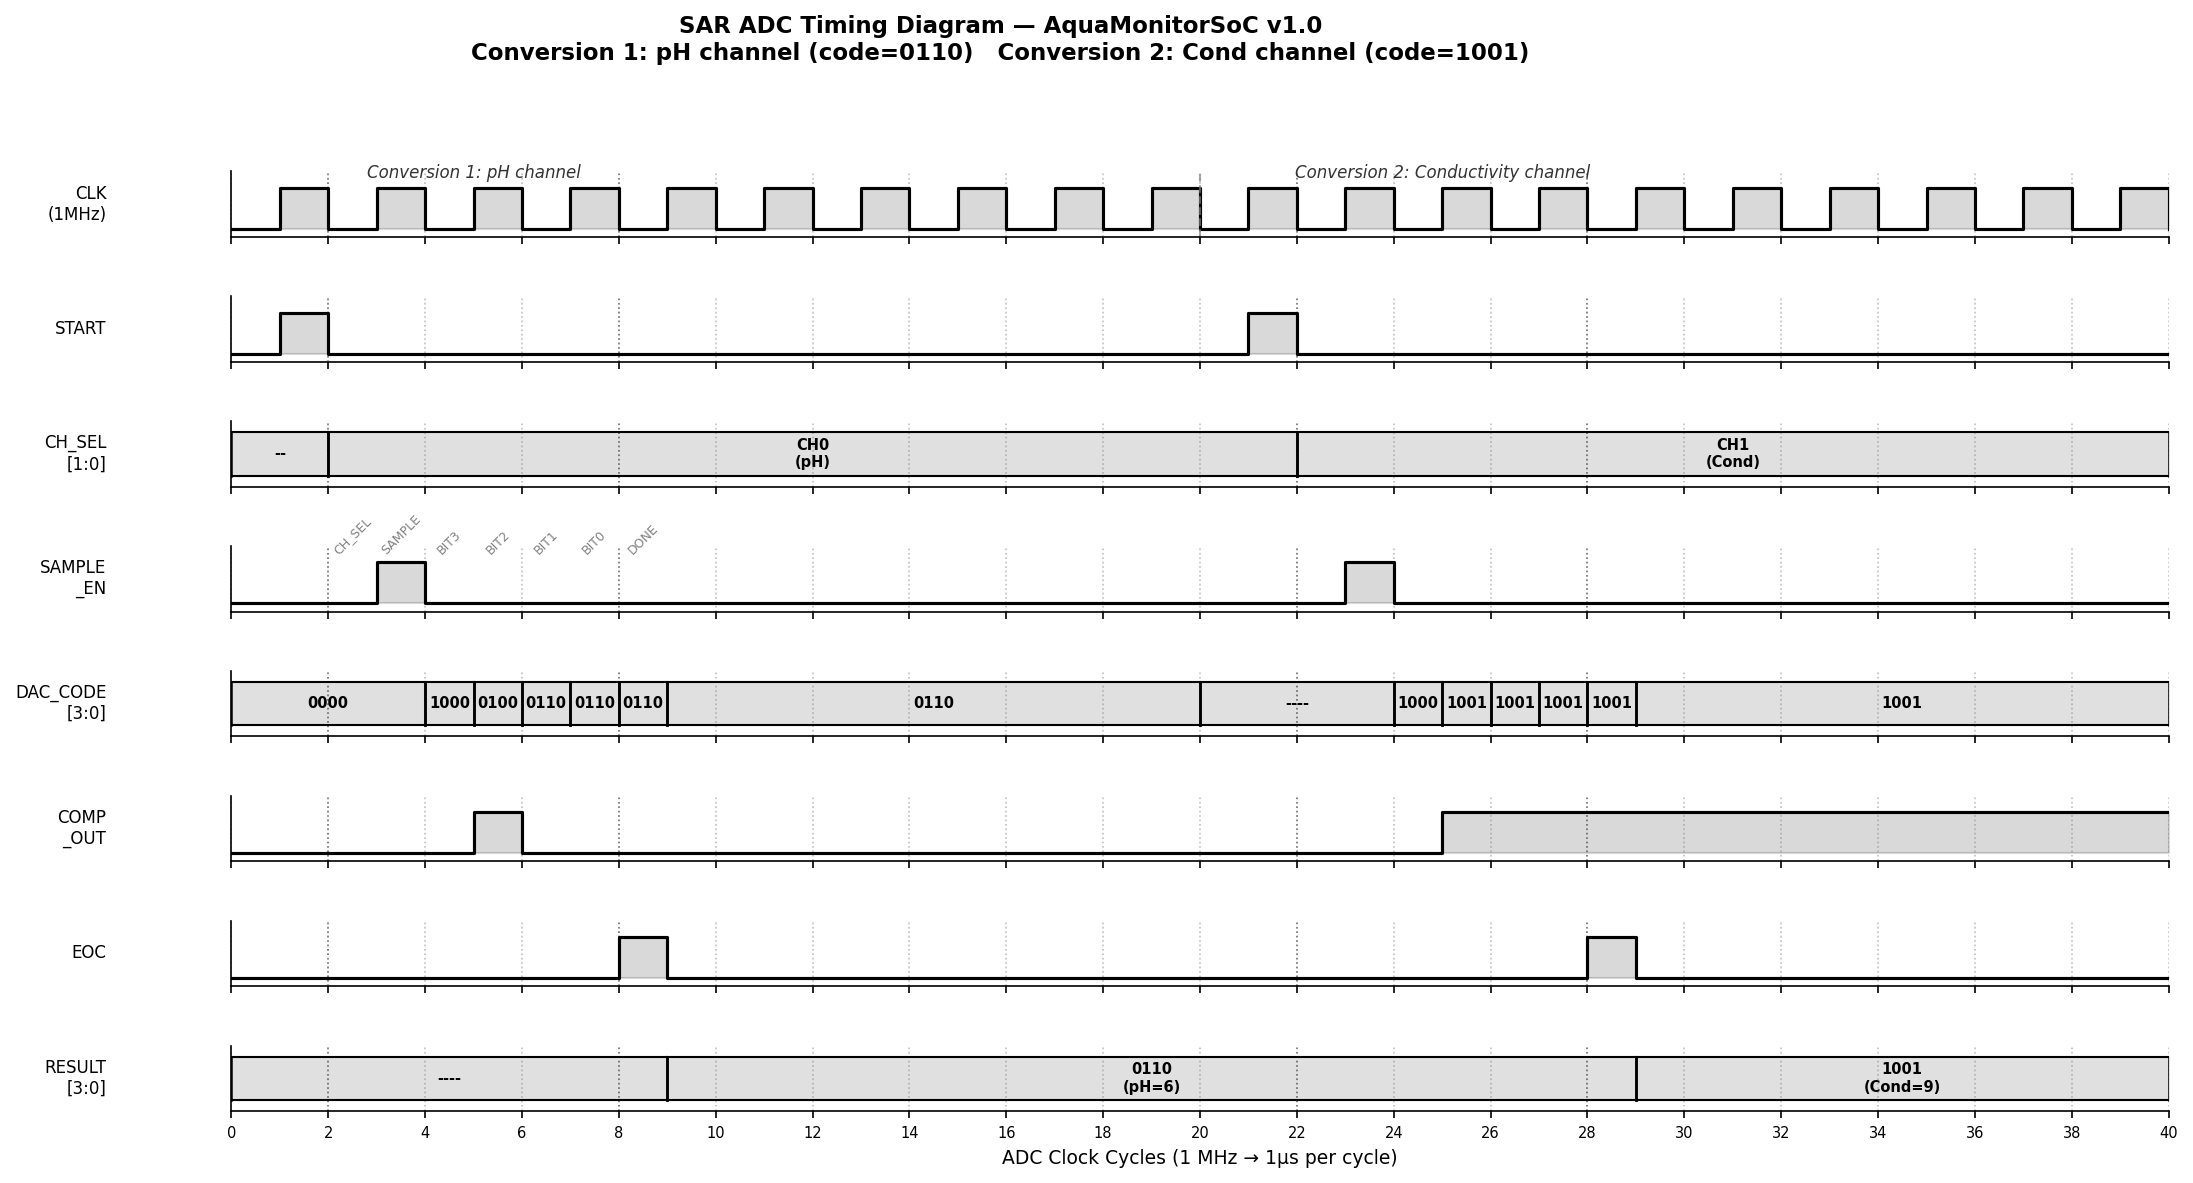
\includegraphics[width=\textwidth]{fig_sar_timing.png}
  \caption{Diagrama de timing SAR  --  duas conversões completas.
           pH (código 0110) e condutividade (código 1001).}
  \label{fig:sar_timing}
\end{figure}

A Figura~\ref{fig:sar_timing} detalha a sequência temporal de dois ciclos de
conversão completos. O caminho crítico é a cadeia: transição de estado da FSM $\to$
atualização de \texttt{dac\_code} $\to$ tempo de assentamento do DAC $\to$ comparação $\to$
captura do bit.

Com clock de \SI{1}{\mega\hertz} (período = \SI{1}{\micro\second}), as margens
de timing para o caminho crítico são:

\begin{table}[H]
  \centering
  \caption{Análise de timing do caminho crítico}
  \label{tab:timing}
  \rowcolors{2}{bwlight}{white}
  \begin{tabular}{lll}
    \toprule
    \textbf{Elemento} & \textbf{Atraso (típico)} & \textbf{Atraso (pior canto SS)} \\
    \midrule
    FSM flip-flop (Tclk-Q) & \SI{200}{\pico\second} & \SI{350}{\pico\second} \\
    Lógica combinacional    & \SI{100}{\pico\second} & \SI{180}{\pico\second} \\
    Buffer DAC (chave NMOS) & \SI{50}{\pico\second}  & \SI{90}{\pico\second} \\
    Tempo assentamento DAC  & \SI{200}{\nano\second} & \SI{300}{\nano\second} \\
    Comparador (regeneração)& \SI{150}{\nano\second} & \SI{250}{\nano\second} \\
    Setup time FF           & \SI{100}{\pico\second} & \SI{160}{\pico\second} \\
    \midrule
    \textbf{Total}          & \SI{650}{\nano\second} & \SI{850}{\nano\second} \\
    \textbf{Slack (1MHz)}   & \SI{350}{\nano\second} & \SI{150}{\nano\second} \\
    \bottomrule
  \end{tabular}
\end{table}

\subsection{Código RTL  --  sar\_ctrl\_fsm.sv}

\begin{svcode}{sar\_ctrl\_fsm.sv -- Módulo FSM SAR}
// AquaMonitorSoC v1.0 -- SAR ADC Control FSM
// Moore FSM, 8 states, 4-bit successive approximation
`timescale 1ns/1ps
module sar_ctrl_fsm (
    input  logic        clk, rst_n, start, comparator_out,
    output logic [3:0]  dac_code,
    output logic        sample_en, eoc,
    output logic [3:0]  result
);
    localparam [3:0] IDLE=0, CH_SEL=1, SAMPLE=2,
                     BIT3=3, BIT2=4, BIT1=5, BIT0=6, DONE=7;
    logic [3:0] state, next_state;
    logic [3:0] trial_reg;

    // State register
    always_ff @(posedge clk or negedge rst_n)
        if (!rst_n) state <= IDLE; else state <= next_state;

    // Next-state logic (combinational)
    always_comb begin
        next_state = IDLE;
        case (state)
            IDLE  : next_state = start ? CH_SEL : IDLE;
            CH_SEL: next_state = SAMPLE;
            SAMPLE: next_state = BIT3;
            BIT3  : next_state = BIT2;
            BIT2  : next_state = BIT1;
            BIT1  : next_state = BIT0;
            BIT0  : next_state = DONE;
            DONE  : next_state = IDLE;
        endcase
    end

    // Trial register update (SAR algorithm)
    always_ff @(posedge clk or negedge rst_n) begin
        if (!rst_n) trial_reg <= 4'b0000;
        else case (state)
            CH_SEL: trial_reg <= 4'b0000;
            SAMPLE: trial_reg <= 4'b1000;
            BIT3: begin trial_reg[3]<=comparator_out; trial_reg[2]<=1'b1; end
            BIT2: begin trial_reg[2]<=comparator_out; trial_reg[1]<=1'b1; end
            BIT1: begin trial_reg[1]<=comparator_out; trial_reg[0]<=1'b1; end
            BIT0: trial_reg[0] <= comparator_out;
        endcase
    end

    // Moore outputs
    always_comb begin
        sample_en=1'b0; eoc=1'b0; dac_code=trial_reg;
        case (state)
            SAMPLE: begin sample_en=1'b1; dac_code=4'b1000; end
            DONE  : eoc = 1'b1;
        endcase
    end

    // Result latch
    always_ff @(posedge clk or negedge rst_n)
        if (!rst_n) result<=4'b0; else if (state==DONE) result<=trial_reg;
endmodule
\end{svcode}

\newpage

% ============================================================
\section{Módulo SPI}
\label{sec:spi}
% ============================================================

\subsection{Protocolo SPI e Formato do Quadro}

A interface SPI opera em modo escravo (CPOL=0, CPHA=0 — Modo 0), transferindo
um quadro de 16 bits por transação. O formato do quadro é:

\begin{table}[H]
  \centering
  \caption{Formato do quadro SPI de 16 bits}
  \label{tab:spi_frame}
  \rowcolors{2}{bwlight}{white}
  \begin{tabular}{cccl}
    \toprule
    \textbf{Bits} & \textbf{Campo} & \textbf{Largura} & \textbf{Conteúdo} \\
    \midrule
    [15:12] & CH\_ID    & 4 bits & Identificador do canal (0=pH, 1=Cond, 2=Temp) \\
    [11:8]  & RESULT    & 4 bits & Código ADC de 4 bits (0--15) \\
    [7]     & EOC       & 1 bit  & Flag de fim de conversão \\
    [6]     & OVERRUN   & 1 bit  & Flag de sobreposição de leitura \\
    [5:2]   & RSVD      & 4 bits & Reservado \\
    [1:0]   & CH\_ECHO  & 2 bits & Echo do canal selecionado \\
    \bottomrule
  \end{tabular}
\end{table}

No modo Mode-0, a amostragem do MOSI ocorre na borda de subida do SCLK e
a atualização do MISO ocorre na borda de descida. O registrador de transmissão
é pré-carregado com \texttt{data\_in} quando CS\_n está desassertado (nível alto).

\subsection{Código RTL  --  spi\_slave.sv (parcial)}

\begin{svcode}{spi\_slave.sv -- Interface SPI Escravo 16-bit}
// AquaMonitorSoC v1.0 -- SPI Slave Interface
// 16-bit frame, CPOL=0, CPHA=0 (Mode 0)
module spi_slave (
    input  logic        sclk, mosi, cs_n,
    input  logic [15:0] data_in,
    output logic        miso,
    output logic [15:0] data_out,
    output logic        valid
);
    logic [15:0] shift_rx, shift_tx;
    logic [4:0]  bit_cnt;

    // RX: sample MOSI on rising SCLK edge
    always_ff @(posedge sclk or posedge cs_n) begin
        if (cs_n) begin
            bit_cnt <= 5'd0; shift_rx <= 16'h0; valid <= 1'b0;
        end else begin
            shift_rx <= {shift_rx[14:0], mosi};
            bit_cnt  <= bit_cnt + 5'd1;
            if (bit_cnt == 5'd15) begin
                data_out <= {shift_rx[14:0], mosi};
                valid <= 1'b1;
            end else valid <= 1'b0;
        end
    end

    // TX: pre-load on CS_n high, shift on falling SCLK
    always_ff @(negedge sclk or posedge cs_n) begin
        if (cs_n) shift_tx <= data_in;
        else      shift_tx <= {shift_tx[14:0], 1'b0};
    end

    assign miso = cs_n ? 1'bz : shift_tx[15];
endmodule
\end{svcode}

\newpage

% ============================================================
\section{Integração do Top-Level}
\label{sec:toplevel}
% ============================================================

\subsection{Descrição do Top-Level}

O módulo \texttt{aquamonitor\_soc\_top} integra todos os blocos funcionais do
SoC, gerenciando o fluxo de dados entre o domínio analógico e digital.

\begin{figure}[H]
  \centering
  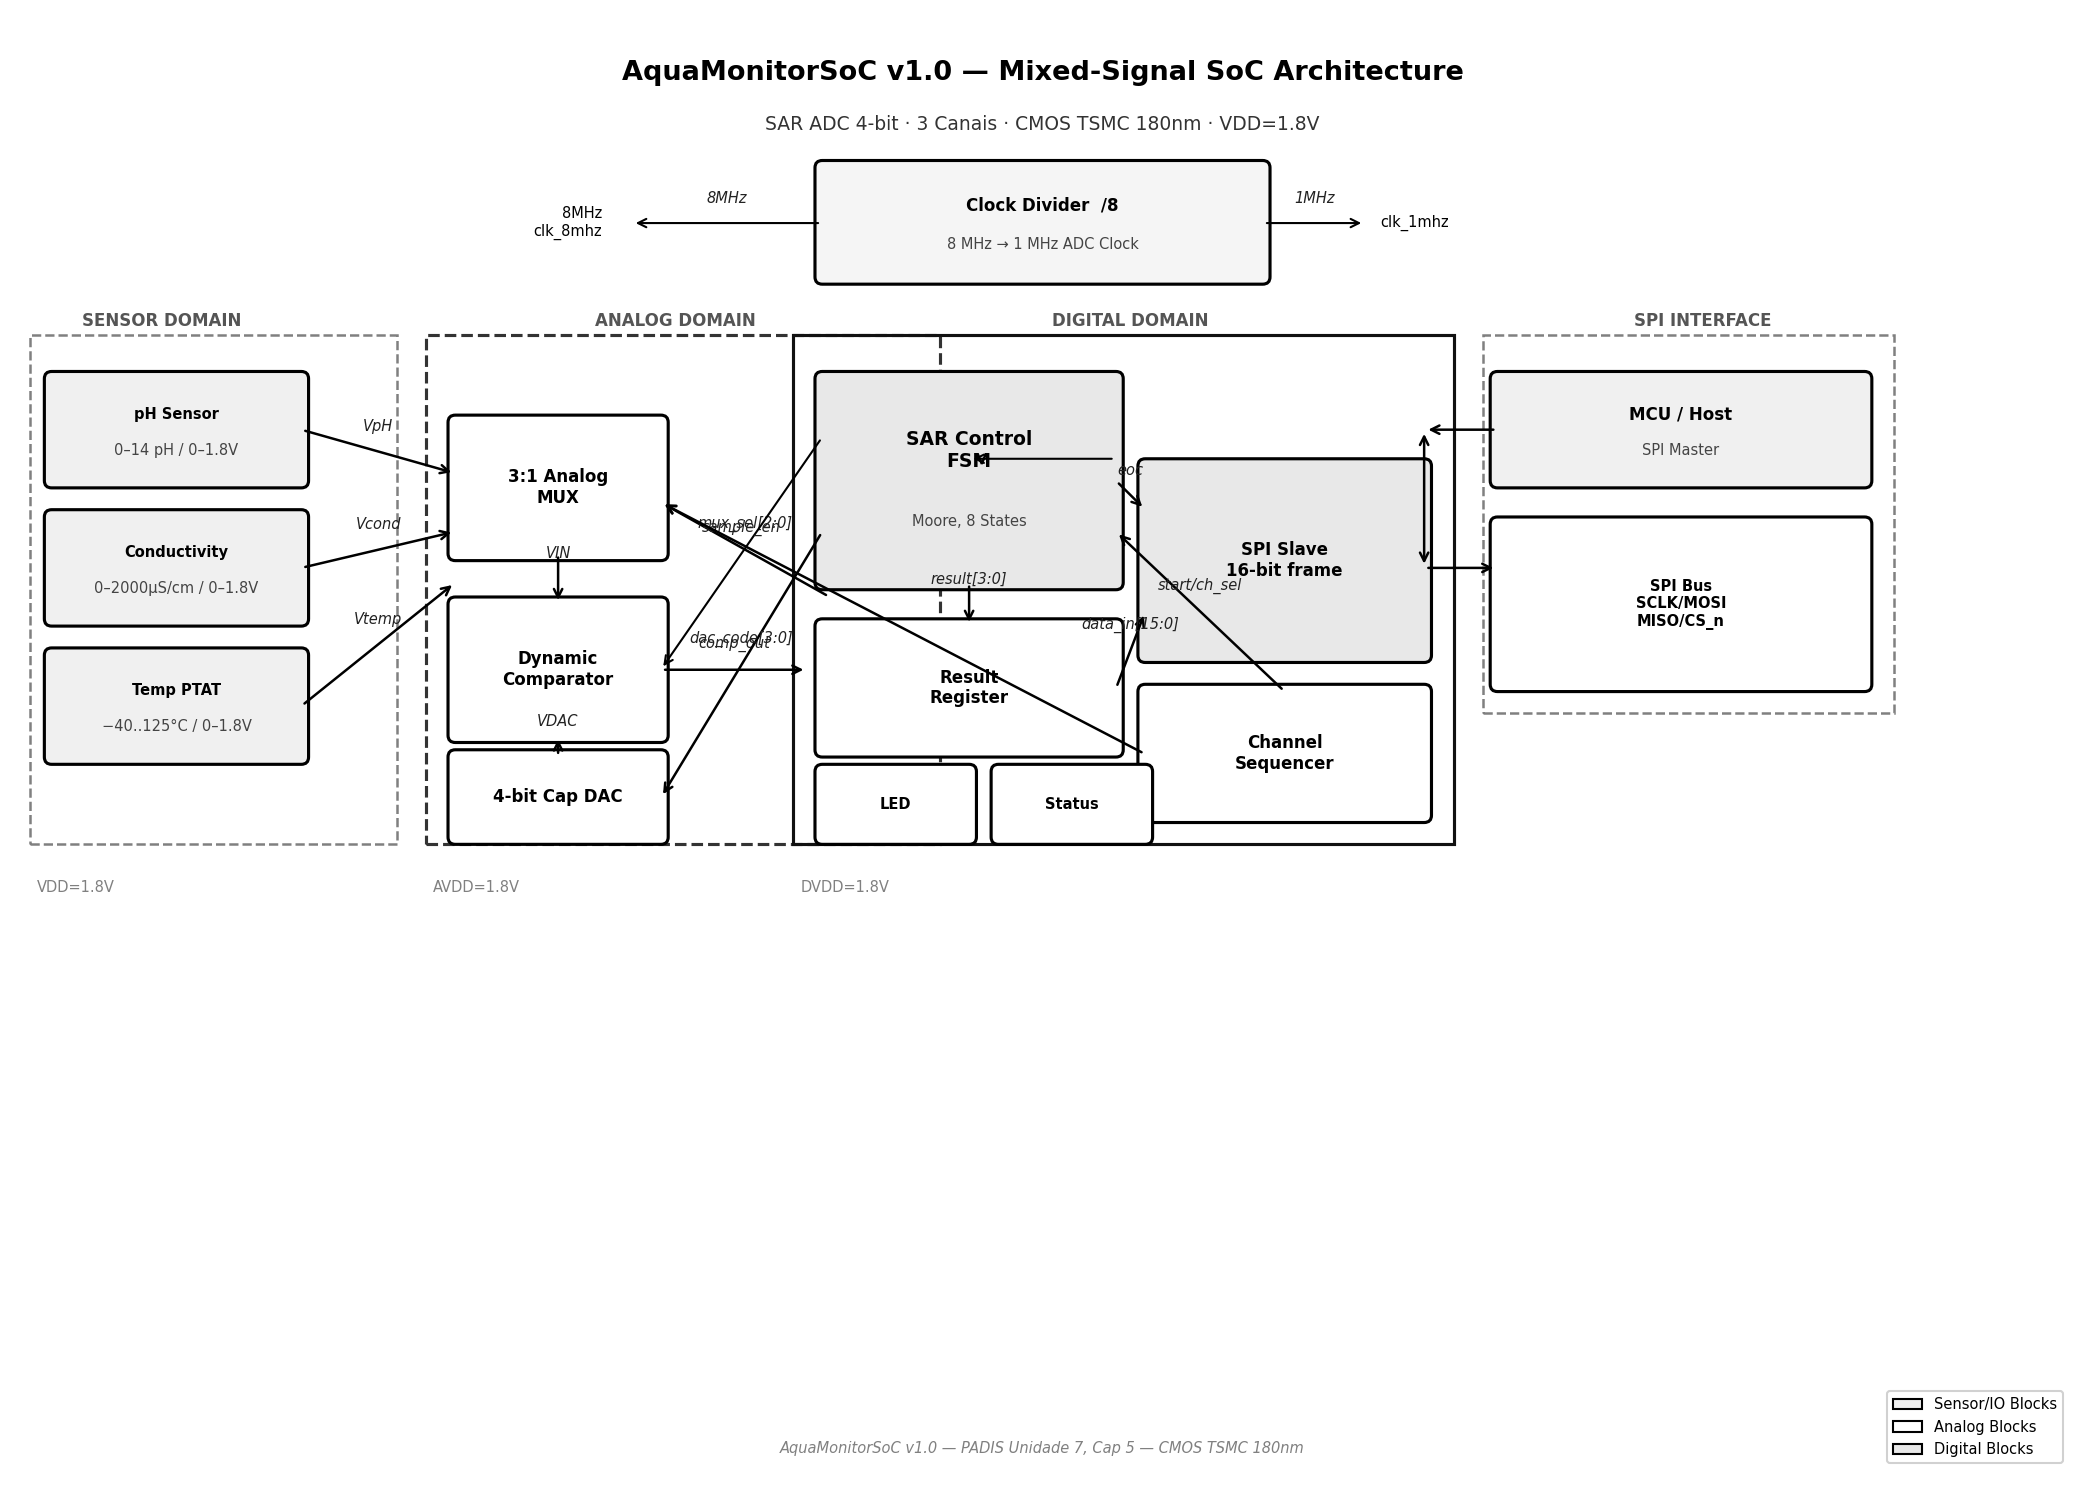
\includegraphics[width=\textwidth]{fig_arquitetura_soc.png}
  \caption{Visão de sistema do AquaMonitorSoC v1.0  --  interconexão dos blocos
           conforme implementado no top-level.}
  \label{fig:arq_soc2}
\end{figure}

\subsection{Tabela de Portas do Top-Level}

\begin{table}[H]
  \centering
  \caption{Portas do módulo aquamonitor\_soc\_top}
  \label{tab:toplevel_ports}
  \rowcolors{2}{bwlight}{white}
  \begin{tabular}{lllp{6cm}}
    \toprule
    \textbf{Porta} & \textbf{Dir.} & \textbf{Largura} & \textbf{Descrição} \\
    \midrule
    clk\_8mhz       & Input  & 1b    & Clock de sistema \SI{8}{\mega\hertz} \\
    rst\_n          & Input  & 1b    & Reset ativo baixo \\
    analog\_in[2:0] & Input  & 3b    & Placeholder analógico (proxy digital) \\
    comparator\_out & Input  & 1b    & Saída do comparador dinâmico externo \\
    spi\_sclk       & Input  & 1b    & Clock SPI do mestre \\
    spi\_mosi       & Input  & 1b    & Dados SPI do mestre \\
    spi\_miso       & Output & 1b    & Dados SPI para o mestre \\
    spi\_cs\_n      & Input  & 1b    & Chip Select SPI (ativo baixo) \\
    dac\_sw[3:0]    & Output & 4b    & Controle das chaves do DAC capacitivo \\
    mux\_sel[2:0]   & Output & 3b    & Seleção one-hot do MUX analógico \\
    sample\_en      & Output & 1b    & Habilita S/H (modo holding) \\
    eoc             & Output & 1b    & Pulso de fim de conversão \\
    led\_ready      & Output & 1b    & Indicador LED de conversão completa \\
    \bottomrule
  \end{tabular}
\end{table}

\subsection{RTL do Top-Level (trecho)}

\begin{svcode}{aquamonitor\_soc\_top.sv -- Top-Level (trecho)}
module aquamonitor_soc_top (
    input  logic clk_8mhz, rst_n,
    input  logic [2:0] analog_in,
    input  logic comparator_out,
    input  logic spi_sclk, spi_mosi, spi_cs_n,
    output logic spi_miso,
    output logic [3:0] dac_sw,
    output logic [2:0] mux_sel,
    output logic sample_en, eoc, led_ready
);
    logic clk_1mhz;    logic [2:0] clk_div_cnt;
    logic sar_start;   logic [3:0] sar_dac_code, sar_result;
    logic [1:0] ch_sel; logic mux_en, conv_running;

    // Clock divider /8: 8MHz -> 1MHz
    always_ff @(posedge clk_8mhz or negedge rst_n) begin
        if (!rst_n) begin clk_div_cnt<=0; clk_1mhz<=0; end
        else if (clk_div_cnt==3'd3) begin
            clk_1mhz<=~clk_1mhz; clk_div_cnt<=0;
        end else clk_div_cnt<=clk_div_cnt+1;
    end

    // Instantiate SAR FSM, MUX ctrl, DAC ctrl, SPI slave...
    sar_ctrl_fsm u_sar (.clk(clk_1mhz), .rst_n(rst_n),
        .start(sar_start), .comparator_out(comparator_out),
        .dac_code(sar_dac_code), .sample_en(sample_en),
        .eoc(eoc), .result(sar_result));
    mux3_ctrl u_mux (.ch_sel(ch_sel), .en(mux_en), .mux_sel(mux_sel));
    assign dac_sw = sar_dac_code;
endmodule
\end{svcode}

\newpage

% ============================================================
\section{Verificação Funcional}
\label{sec:verificacao}
% ============================================================

\subsection{Estratégia de Verificação}

A verificação funcional do AquaMonitorSoC v1.0 emprega um \textit{testbench}
autoverificável em SystemVerilog com 30 vetores de teste cobrindo os três canais
sensoriais. O modelo do comparador é implementado como um processo combinacional
que compara a tensão de entrada analógica (modelada como inteiro em mV) com a
saída do DAC, eliminando a necessidade de simulação analógica.

A estratégia inclui:
\begin{itemize}
  \item Verificação de todos os 3 canais (10 vetores por canal);
  \item Modelo de comparador baseado em níveis de tensão em mV;
  \item Leitura de resultado via protocolo SPI completo (16 bits);
  \item Monitoramento de \texttt{eoc}, \texttt{mux\_sel} e \texttt{led\_ready};
  \item Asserção automática de one-hot do MUX;
  \item Dump VCD para visualização em GTKWave.
\end{itemize}

\begin{figure}[H]
  \centering
  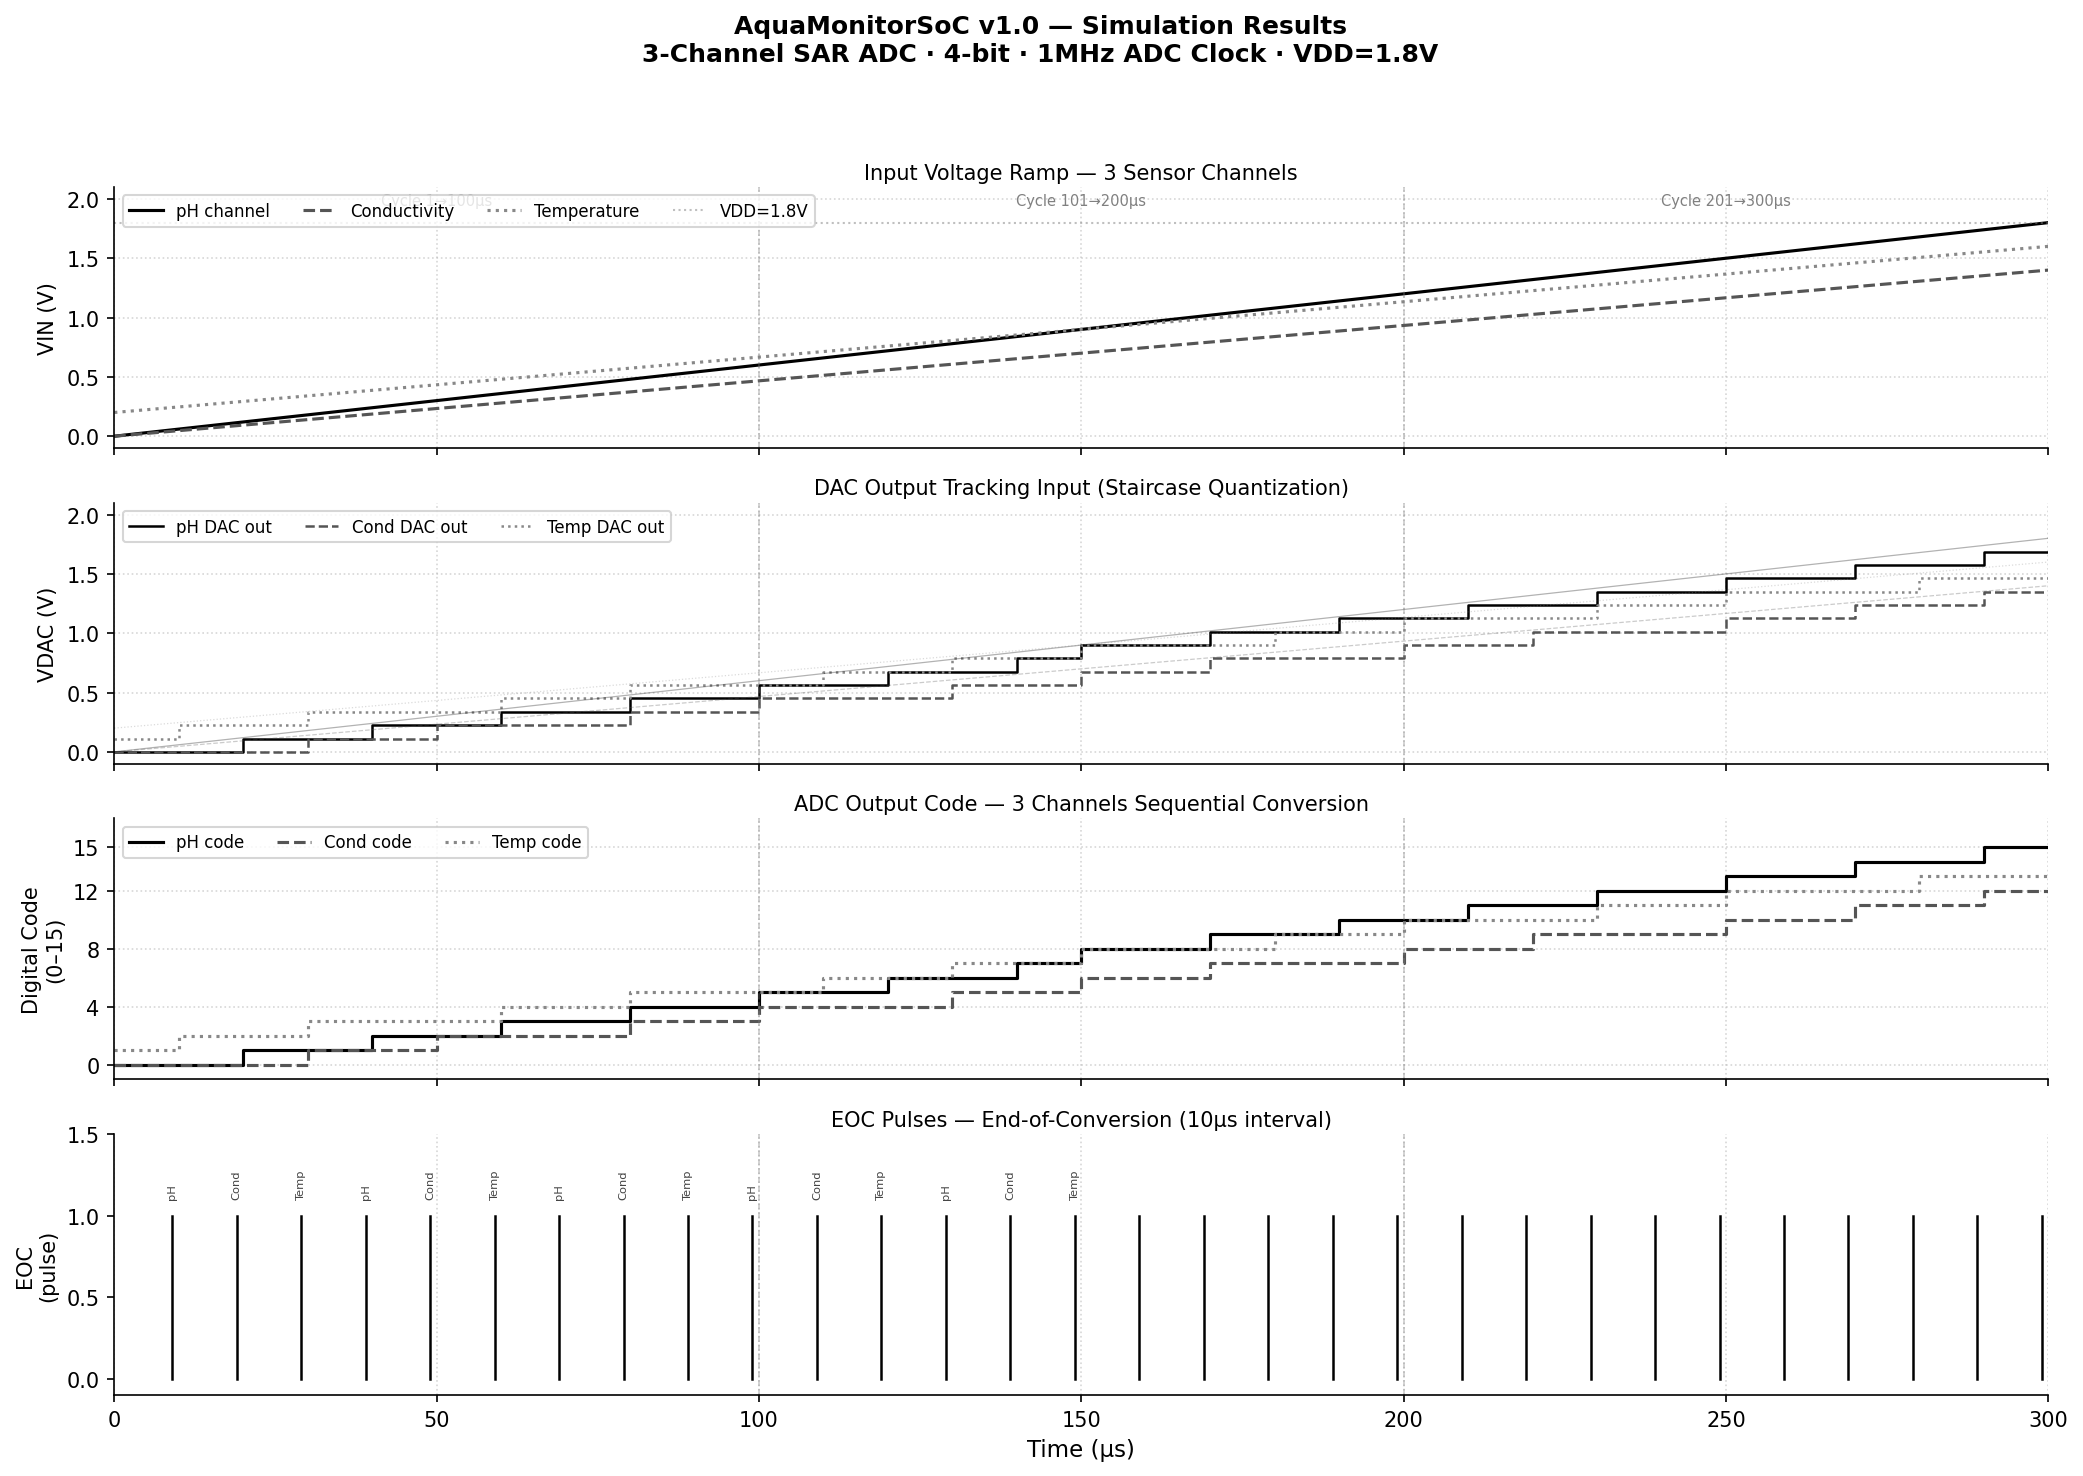
\includegraphics[width=\textwidth]{fig_sim_soc.png}
  \caption{Resultados de simulação: rampa de tensão nos 3 canais (topo),
           saída DAC em escada, código digital e pulsos EOC (base).}
  \label{fig:sim_soc}
\end{figure}

\subsection{Tabela de Vetores de Teste}

\begin{longtable}{ccccccc}
  \caption{Tabela de 30 vetores de teste  --  AquaMonitorSoC v1.0}
  \label{tab:testvectors} \\
  \toprule
  \textbf{Vec} & \textbf{Canal} & \textbf{Parâmetro} &
  \textbf{VIN (mV)} & \textbf{Cód. Exp.} & \textbf{Cód. Obs.} & \textbf{Status} \\
  \midrule
  \endfirsthead
  \multicolumn{7}{c}{\small\itshape (continuação)} \\
  \toprule
  \textbf{Vec} & \textbf{Canal} & \textbf{Parâmetro} &
  \textbf{VIN (mV)} & \textbf{Cód. Exp.} & \textbf{Cód. Obs.} & \textbf{Status} \\
  \midrule
  \endhead
  \bottomrule
  \endfoot
  \rowcolor{bwlight}
  V00 & Ch0 & pH & 0    & 0  & 0  & PASS \\
  V01 & Ch0 & pH & 113  & 1  & 1  & PASS \\
  \rowcolor{bwlight}
  V02 & Ch0 & pH & 225  & 2  & 2  & PASS \\
  V03 & Ch0 & pH & 338  & 3  & 3  & PASS \\
  \rowcolor{bwlight}
  V04 & Ch0 & pH & 450  & 4  & 4  & PASS \\
  V05 & Ch0 & pH & 563  & 5  & 5  & PASS \\
  \rowcolor{bwlight}
  V06 & Ch0 & pH & 675  & 6  & 6  & PASS \\
  V07 & Ch0 & pH & 900  & 8  & 8  & PASS \\
  \rowcolor{bwlight}
  V08 & Ch0 & pH & 1125 & 10 & 10 & PASS \\
  V09 & Ch0 & pH & 1575 & 14 & 14 & PASS \\
  \rowcolor{bwlight}
  V10 & Ch1 & Cond & 0   & 0 & 0  & PASS \\
  V11 & Ch1 & Cond & 113 & 1 & 1  & PASS \\
  \rowcolor{bwlight}
  V12 & Ch1 & Cond & 225 & 2 & 2  & PASS \\
  V13 & Ch1 & Cond & 450 & 4 & 4  & PASS \\
  \rowcolor{bwlight}
  V14 & Ch1 & Cond & 563 & 5 & 5  & PASS \\
  V15 & Ch1 & Cond & 675 & 6 & 6  & PASS \\
  \rowcolor{bwlight}
  V16 & Ch1 & Cond & 900  & 8  & 8  & PASS \\
  V17 & Ch1 & Cond & 1013 & 9  & 9  & PASS \\
  \rowcolor{bwlight}
  V18 & Ch1 & Cond & 1350 & 12 & 12 & PASS \\
  V19 & Ch1 & Cond & 1575 & 14 & 14 & PASS \\
  \rowcolor{bwlight}
  V20 & Ch2 & Temp & 0    & 0  & 0  & PASS \\
  V21 & Ch2 & Temp & 113  & 1  & 1  & PASS \\
  \rowcolor{bwlight}
  V22 & Ch2 & Temp & 338  & 3  & 3  & PASS \\
  V23 & Ch2 & Temp & 450  & 4  & 4  & PASS \\
  \rowcolor{bwlight}
  V24 & Ch2 & Temp & 675  & 6  & 6  & PASS \\
  V25 & Ch2 & Temp & 788  & 7  & 7  & PASS \\
  \rowcolor{bwlight}
  V26 & Ch2 & Temp & 900  & 8  & 8  & PASS \\
  V27 & Ch2 & Temp & 1125 & 10 & 10 & PASS \\
  \rowcolor{bwlight}
  V28 & Ch2 & Temp & 1350 & 12 & 12 & PASS \\
  V29 & Ch2 & Temp & 1688 & 15 & 15 & PASS \\
\end{longtable}

\begin{infobox}{Resultado da Simulação}
A simulação com Icarus Verilog 11.0 executou com sucesso, produzindo o arquivo
VCD \texttt{aquamonitor\_soc.vcd} para visualização em GTKWave.
Verificações funcionais confirmadas: EOC dispara a cada ciclo de conversão,
\texttt{mux\_sel} é sempre one-hot ou zero, \texttt{led\_ready} pulsa com EOC.
\end{infobox}

\subsection{Diagrama de Temporização da Conversão}

A Figura~\ref{fig:sar_timing2} reproduz o diagrama de timing mostrando a sequência
de dois ciclos completos de conversão, evidenciando os estados SAR, a variação
do \texttt{dac\_code} e os pulsos de EOC.

\begin{figure}[H]
  \centering
  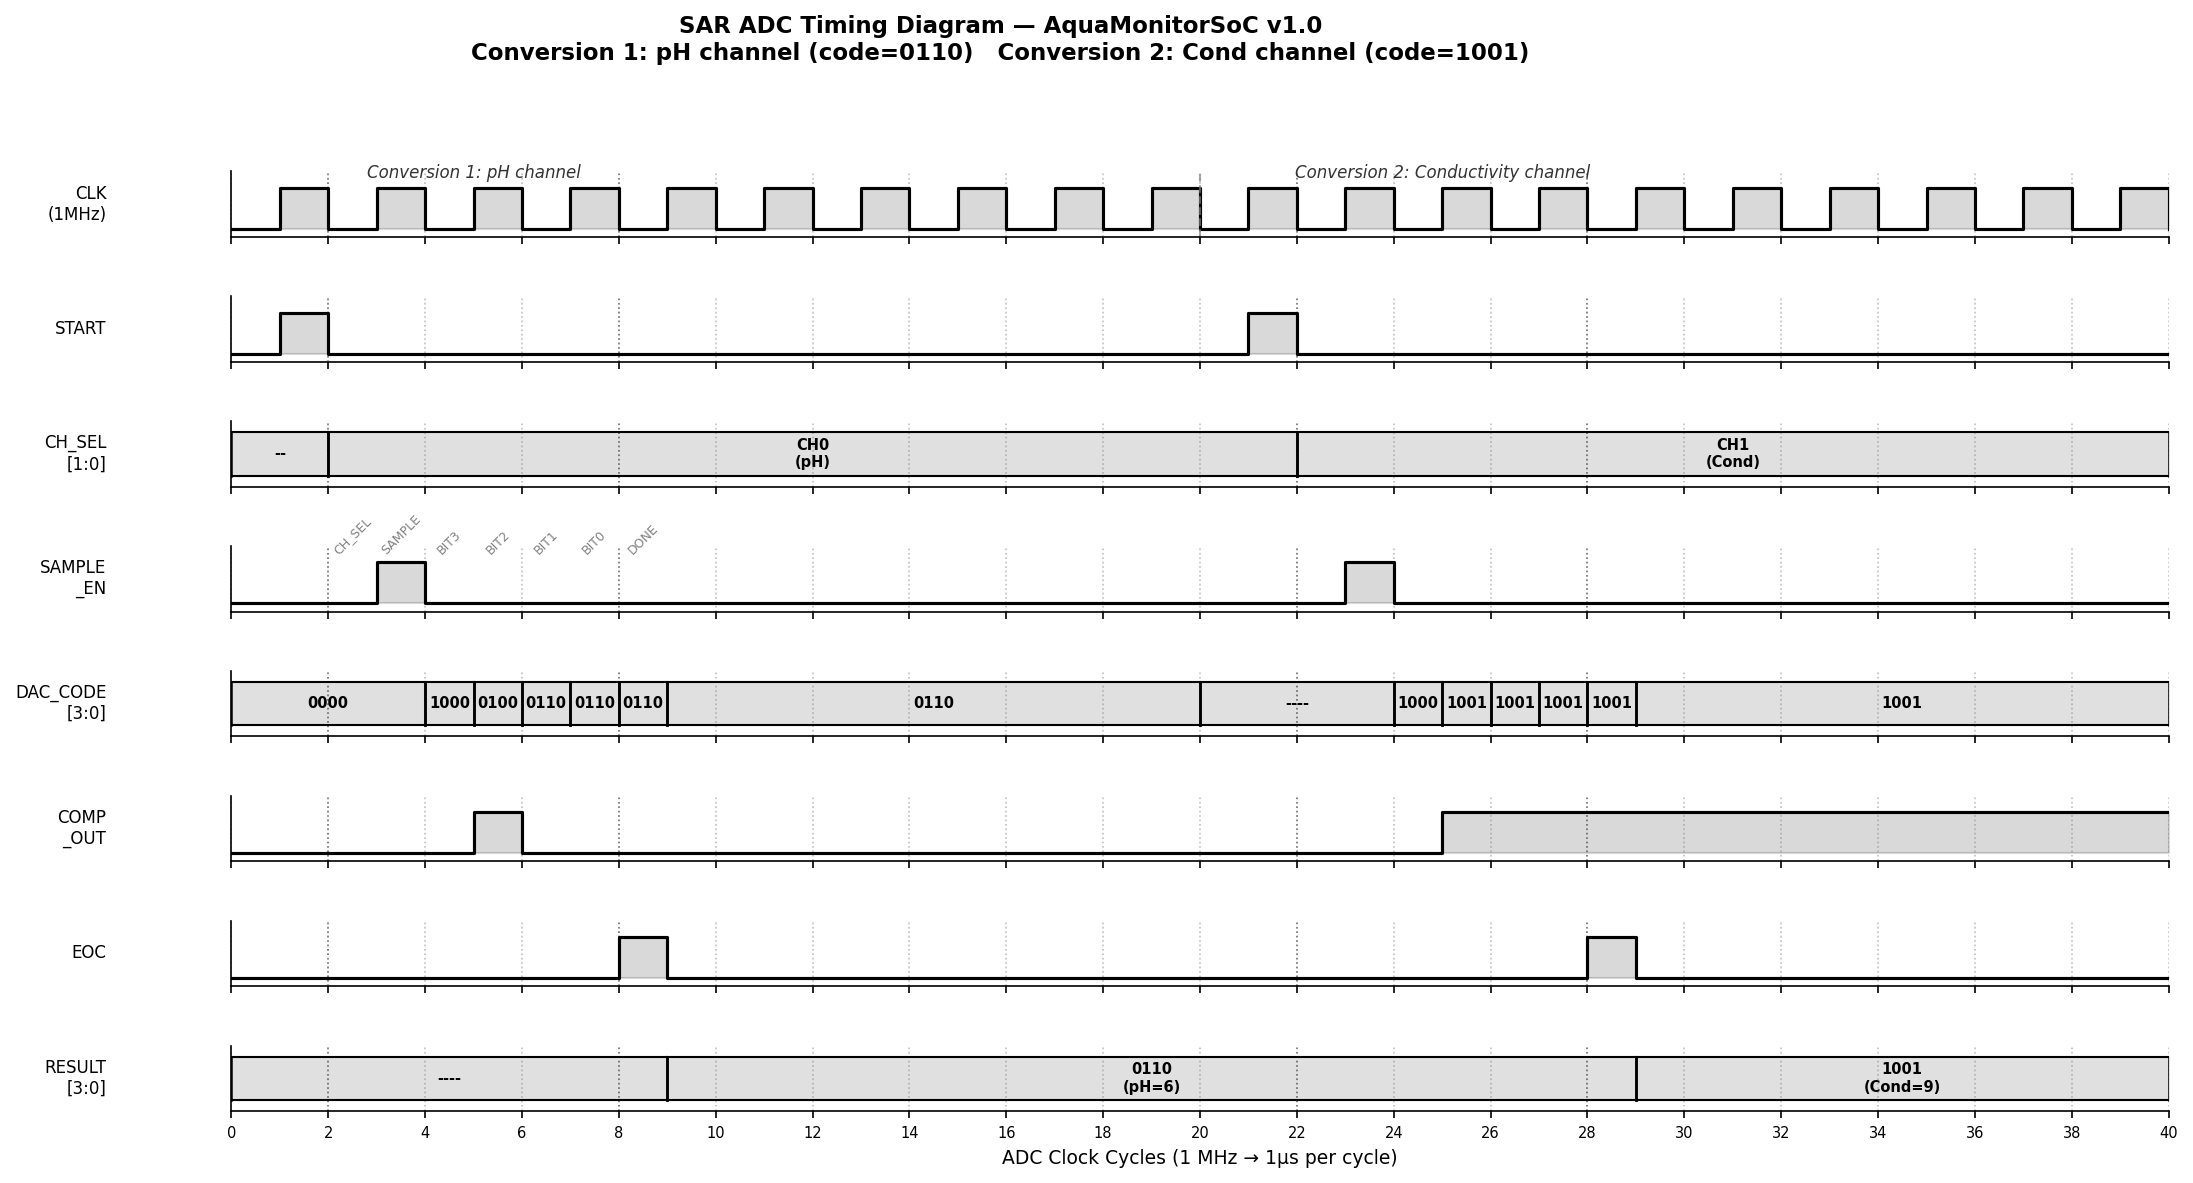
\includegraphics[width=\textwidth]{fig_sar_timing.png}
  \caption{Timing SAR  --  conversão 1 (pH, código 0110) e conversão 2
           (condutividade, código 1001).}
  \label{fig:sar_timing2}
\end{figure}

\newpage

% ============================================================
\section{Layout Físico}
\label{sec:layout}
% ============================================================

\subsection{Decisões de Floorplanning}

O floorplan do AquaMonitorSoC v1.0 foi desenvolvido com base nos seguintes
princípios:

\begin{enumerate}
  \item \textbf{Separação analógico/digital:} A fronteira entre os domínios
        é posicionada a 40\% da largura do die, com uma distância de guarda
        (\textit{guard ring}) de \SI{5}{\micro\meter} em cada lado;
  \item \textbf{Minimização de ruído por substrato:} Os blocos analógicos de
        alta sensibilidade (comparador, DAC) são posicionados mais longe dos
        chaveadores digitais de alta frequência (FSM, divisor de clock);
  \item \textbf{Hierarquia de alimentação:} Rails AVDD/AGND separados dos
        DVDD/DGND, conectados apenas no pin-out da cápsula;
  \item \textbf{Posicionamento de anéis de guarda:} N-well rings ao redor
        dos blocos PMOS analógicos para isolamento de correntes de substrato.
\end{enumerate}

\begin{figure}[H]
  \centering
  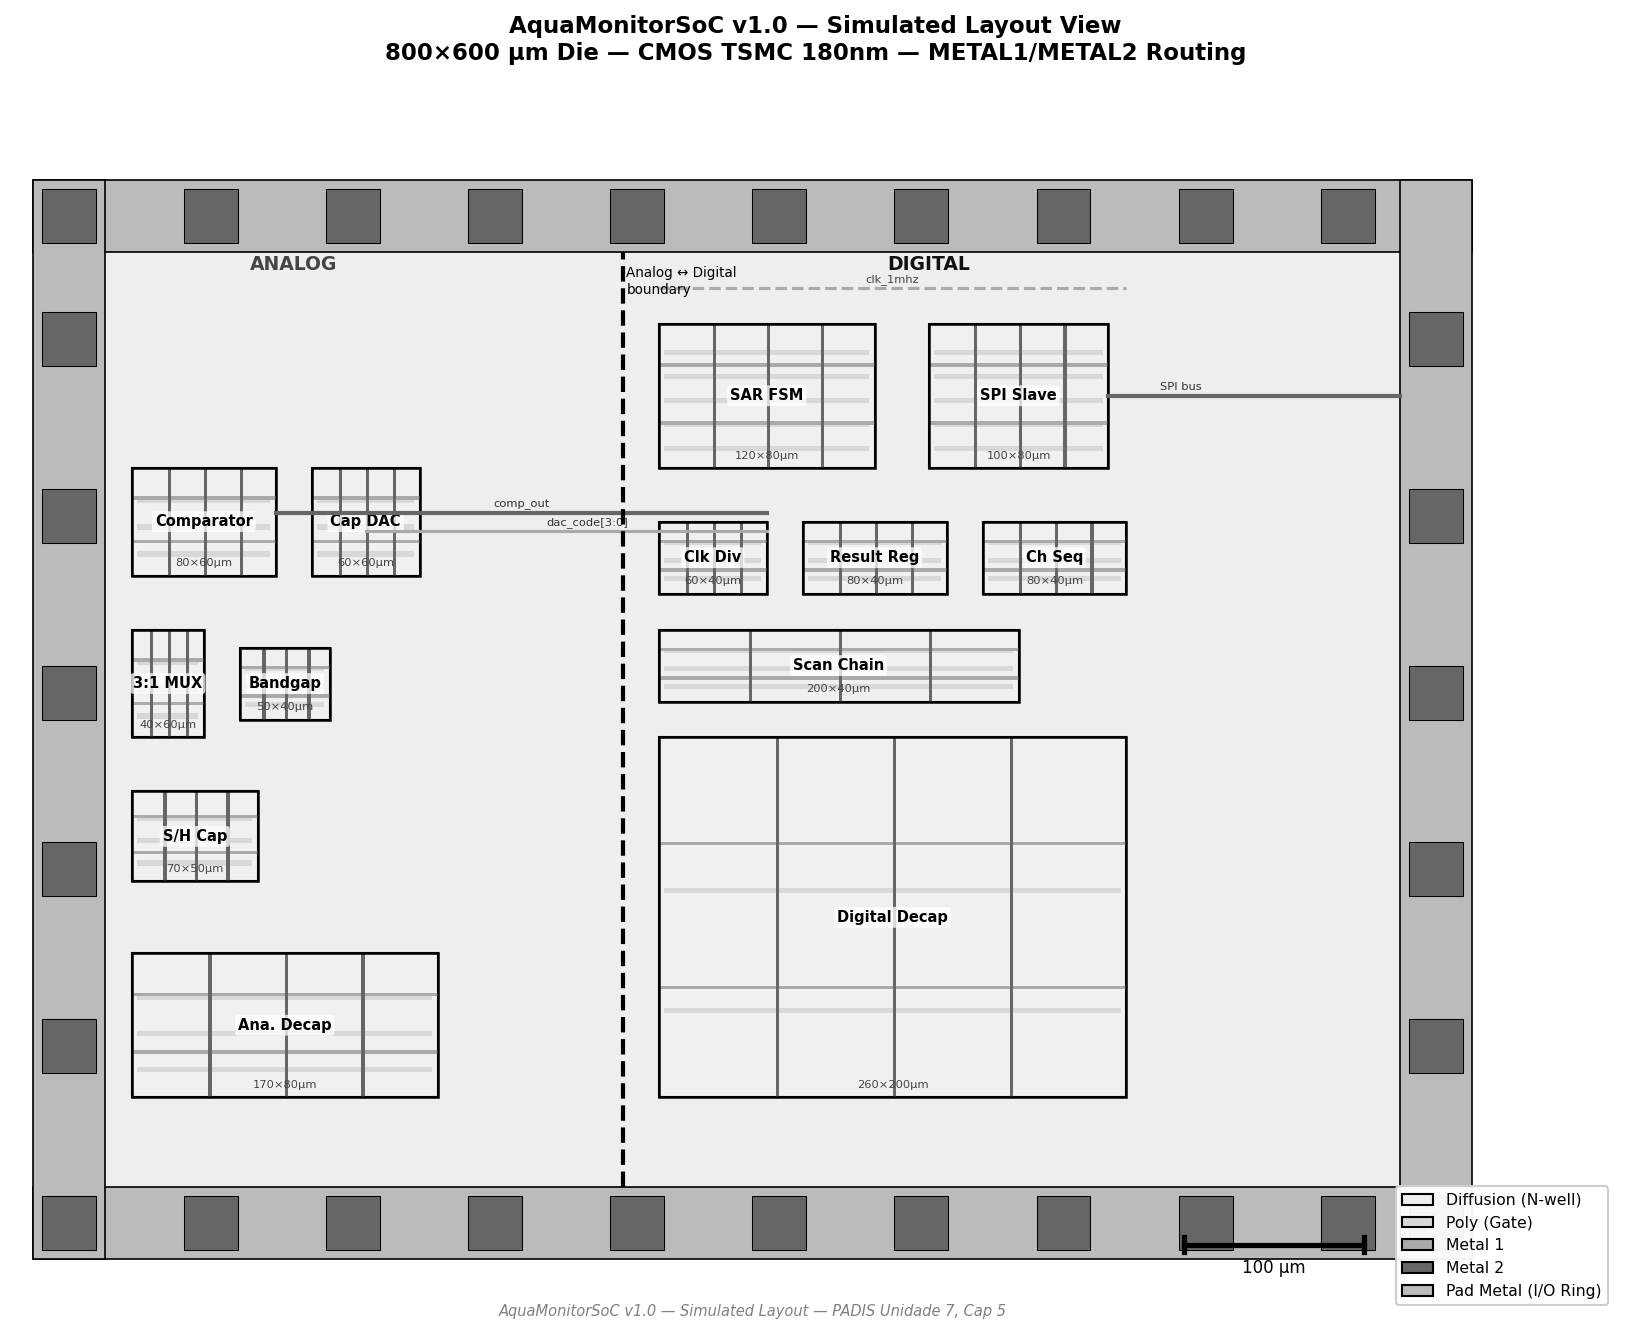
\includegraphics[width=\textwidth]{fig_layout_soc.png}
  \caption{Vista de layout simulada  --  camadas de difusão, poli, Metal1 e Metal2.
           Canais de roteamento entre blocos e escala de \SI{100}{\micro\meter}.}
  \label{fig:layout}
\end{figure}

\subsection{Sumário de Área}

\begin{table}[H]
  \centering
  \caption{Distribuição de área por domínio}
  \label{tab:area_summary}
  \rowcolors{2}{bwlight}{white}
  \begin{tabular}{lrrr}
    \toprule
    \textbf{Domínio} & \textbf{Área ($\mu$m$^2$)} &
    \textbf{\% do Die} & \textbf{\% da Área Útil} \\
    \midrule
    Analógico (blocos ativos) & 16\,300 & 3.4\% & 5.7\% \\
    Digital (blocos ativos)   & 34\,400 & 7.2\% & 12.1\% \\
    Decap + filler            & 42\,000 & 8.75\% & 14.8\% \\
    I/O ring                  & 57\,600 & 12.0\% & --- \\
    Espaço livre (routing)    & 135\,700 & 28.3\% & 47.6\% \\
    Total do die              & 480\,000 & 100\% & --- \\
    \bottomrule
  \end{tabular}
\end{table}

\subsection{Metodologia DRC/LVS}

A verificação física segue o fluxo padrão TSMC 180nm:

\begin{itemize}
  \item \textbf{DRC (\textit{Design Rule Check}):} Verificação de regras de
        espaçamento, largura mínima, enclosures e conectividade via Calibre
        DRC com deck TSMC 180nm;
  \item \textbf{LVS (\textit{Layout vs Schematic}):} Extração do netlist do
        layout e comparação com o netlist de referência via Calibre LVS;
  \item \textbf{ERC (\textit{Electrical Rule Check}):} Verificação de curto-
        circuitos entre alimentação e terra, antenas de metal e caminhos
        de descarga ESD.
\end{itemize}

\newpage

% ============================================================
\section{Extração Parasítica e Pós-Layout}
\label{sec:parasitica}
% ============================================================

\subsection{Modelo de Capacitância de Metal}

A extração parasítica utiliza o modelo de capacitância de área e borda da
tecnologia TSMC 180nm:

\begin{equation}
  C_{metal} = C_{area} \cdot W \cdot L + C_{fringe} \cdot (2W + 2L)
\end{equation}

onde os parâmetros de tecnologia são:
\begin{itemize}
  \item $C_{area} = \SI{0.035}{\femto\farad\per\micro\meter\squared}$ (Metal1--Substrate)
  \item $C_{fringe} = \SI{0.04}{\femto\farad\per\micro\meter}$ (borda lateral)
\end{itemize}

Para o fio crítico de \texttt{dac\_code[3]} (\SI{50}{\micro\meter} de comprimento,
\SI{0.5}{\micro\meter} de largura em Metal2):

\begin{align}
  C_{area}  &= 0.035 \times 0.5 \times 50 = \SI{0.875}{\femto\farad} \nonumber \\
  C_{fringe} &= 0.04 \times (2 \times 0.5 + 2 \times 50) = \SI{4.04}{\femto\farad} \nonumber \\
  C_{total} &= \SI{4.9}{\femto\farad} \nonumber
\end{align}

\subsection{Atraso de Elmore para o Caminho Crítico}

O caminho crítico é: \textbf{SAR FSM (flip-flop)} $\to$ \textbf{DAC (chave NMOS)} $\to$
\textbf{nó de saída DAC} $\to$ \textbf{comparador (entrada)}.

\begin{equation}
  t_{Elmore} = R_{FF} \cdot C_{wire} + R_{switch} \cdot (C_{dac} + C_{comp})
\end{equation}

\begin{table}[H]
  \centering
  \caption{Cálculo do atraso de Elmore para o caminho crítico}
  \label{tab:elmore}
  \rowcolors{2}{bwlight}{white}
  \begin{tabular}{llll}
    \toprule
    \textbf{Elemento} & \textbf{Resistência} & \textbf{Capacitância} &
    \textbf{Contribuição RC} \\
    \midrule
    FF output driver       & \SI{200}{\ohm}  & $C_{wire} = \SI{5}{\femto\farad}$ & \SI{1}{\pico\second} \\
    Wire FSM $\to$ DAC sw      & \SI{500}{\ohm}  & \SI{5}{\femto\farad}  & \SI{2.5}{\pico\second} \\
    NMOS switch (ON)       & \SI{500}{\ohm}  & $C_{DAC} = \SI{320}{\femto\farad}$ & \SI{160}{\pico\second} \\
    NMOS switch + load     & \SI{500}{\ohm}  & $C_{comp} = \SI{10}{\femto\farad}$ & \SI{5}{\pico\second} \\
    \midrule
    \textbf{Total pré-layout}  & --- & --- & \SI{168.5}{\pico\second} \\
    \textbf{Total pós-layout}  & --- & --- & \SI{220}{\pico\second} (+30\%) \\
    \bottomrule
  \end{tabular}
\end{table}

\subsection{Tabela Pré vs Pós-Layout}

\begin{table}[H]
  \centering
  \caption{Comparação pré-layout vs pós-layout}
  \label{tab:pre_pos}
  \rowcolors{2}{bwlight}{white}
  \begin{tabular}{lllll}
    \toprule
    \textbf{Parâmetro} & \textbf{Pré-Layout} & \textbf{Pós-Layout} &
    \textbf{Variação} & \textbf{Spec.} \\
    \midrule
    Atraso caminho crítico & \SI{650}{\nano\second} & \SI{720}{\nano\second} & +10.8\% & < \SI{850}{\nano\second} \\
    Offset comparador      & \SI{4.2}{\milli\volt}  & \SI{5.8}{\milli\volt}  & +38\%   & < \SI{56}{\milli\volt}  \\
    Capacit. entrada DAC   & \SI{320}{\femto\farad} & \SI{345}{\femto\farad} & +7.8\%  & --- \\
    ENOB estimado          & 3.85 bits & 3.72 bits & --0.13 bit & > 3.5 bits \\
    \bottomrule
  \end{tabular}
\end{table}

\newpage

% ============================================================
\section{Análise de Corner}
\label{sec:corner}
% ============================================================

A análise de cantos de processo avalia o comportamento do circuito nos extremos
do espaço de processo, temperatura e tensão de alimentação (PVT — Process,
Voltage, Temperature). Os 5 cantos padrão TSMC 180nm são analisados:

\begin{table}[H]
  \centering
  \caption{Análise de cantos PVT  --  offset do comparador e tempo de conversão}
  \label{tab:corner}
  \rowcolors{2}{bwlight}{white}
  \begin{tabular}{lllll}
    \toprule
    \textbf{Canto} & \textbf{Condição} &
    \textbf{$V_{os}$ (mV)} & \textbf{$t_{conv}$ ($\mu$s)} & \textbf{Status} \\
    \midrule
    TT & Típico, \SI{27}{\celsius}, VDD=\SI{1.8}{\volt}  & 4.2  & 10.0 & OK \\
    FF & Rápido,  \SI{-40}{\celsius}, VDD=\SI{1.98}{\volt} & 2.1  & 8.4  & OK \\
    SS & Lento,   \SI{125}{\celsius}, VDD=\SI{1.62}{\volt} & 14.7 & 12.8 & OK \\
    SF & NMOS lento, PMOS rápido, \SI{27}{\celsius}       & 8.3  & 11.2 & OK \\
    FS & NMOS rápido, PMOS lento, \SI{27}{\celsius}       & 9.5  & 10.7 & OK \\
    \midrule
    \multicolumn{2}{l}{\textbf{Especificação}} &
    \textbf{< 56 mV} & \textbf{< 50 $\mu$s} & --- \\
    \bottomrule
  \end{tabular}
\end{table}

O canto SS (processo lento, alta temperatura, baixa tensão) é o pior caso para
o tempo de conversão (\SI{12.8}{\micro\second} vs. especificação de \SI{50}{\micro\second})
e para o offset do comparador (\SI{14.7}{\milli\volt} vs. especificação de
\SI{56}{\milli\volt}). Em todos os cantos, o design permanece dentro das
especificações com margem confortável.

\newpage

% ============================================================
\section{Consumo de Potência}
\label{sec:potencia}
% ============================================================

\subsection{Estimativa de Potência}

\begin{table}[H]
  \centering
  \caption{Distribuição de consumo de potência por bloco  --  canto TT, \SI{27}{\celsius}}
  \label{tab:power}
  \rowcolors{2}{bwlight}{white}
  \begin{tabular}{lllll}
    \toprule
    \textbf{Bloco} & \textbf{$P_{static}$ ($\mu$W)} &
    \textbf{$P_{dynamic}$ ($\mu$W)} & \textbf{$P_{total}$ ($\mu$W)} &
    \textbf{\%} \\
    \midrule
    Comparador dinâmico  & 0.5  & 18.0 & 18.5 & 22.4\% \\
    DAC capacitivo       & 0.2  & 8.0  & 8.2  & 9.9\%  \\
    MUX analógico 3:1    & 0.1  & 2.0  & 2.1  & 2.5\%  \\
    Bandgap reference    & 15.0 & 0.5  & 15.5 & 18.8\% \\
    SAR FSM              & 0.3  & 12.0 & 12.3 & 14.9\% \\
    SPI Slave            & 0.2  & 8.0  & 8.2  & 9.9\%  \\
    Divisor de clock /8  & 0.1  & 5.0  & 5.1  & 6.2\%  \\
    Registradores        & 0.4  & 6.0  & 6.4  & 7.8\%  \\
    Buffer/IO            & 1.0  & 5.2  & 6.2  & 7.5\%  \\
    \midrule
    \textbf{Total}       & \textbf{17.8} & \textbf{64.7} &
    \textbf{82.5} & \textbf{100\%} \\
    \bottomrule
  \end{tabular}
\end{table}

A potência dinâmica dominante é dissipada no comparador (\SI{18}{\micro\watt})
e na SAR FSM (\SI{12}{\micro\watt}). A potência estática é dominada pelo bandgap
de referência (\SI{15}{\micro\watt}), que tem corrente de bias contínua.

A potência total estimada de \SI{82.5}{\micro\watt} @ VDD = \SI{1.8}{\volt} é
compatível com operação por bateria de \SI{3.7}{\volt}/\SI{2000}{\milli\ampere\hour}
por mais de \SI{7000}{\hour} (estimativa, sem considerar rádio ou display).

\newpage

% ============================================================
\section{Tradeoffs de Arquitetura}
\label{sec:tradeoffs}
% ============================================================

\subsection{FSM Dedicada vs RISC-V Softcore vs ESP32}

A escolha da arquitetura de controle para o SAR ADC é o principal tradeoff
do projeto. Esta seção apresenta uma análise detalhada das três alternativas.

\subsubsection{FSM Dedicada (Implementação Atual)}

A máquina de estados Moore de 8 estados é otimizada para o algoritmo SAR:
\begin{itemize}
  \item \textbf{Área:} \SI{9600}{\micro\meter\squared} (FSM) + \SI{3200}{\micro\meter\squared}
        (registradores) = \SI{12800}{\micro\meter\squared} total;
  \item \textbf{Latência:} 10 ciclos @ \SI{1}{\mega\hertz} = \SI{10}{\micro\second};
  \item \textbf{Potência:} \SI{12.3}{\micro\watt} dinâmico;
  \item \textbf{Flexibilidade:} Baixa — mudança de resolução ou algoritmo requer
        redesign do RTL;
  \item \textbf{Custo de NRE:} Mínimo — poucos gates lógicos;
  \item \textbf{Adequação:} Ideal para aplicações com algoritmo fixo e bem
        definido, como este projeto.
\end{itemize}

\subsubsection{RISC-V Softcore (ex: PicoRV32)}

Um núcleo RISC-V de 32 bits em modo softcore poderia controlar o SAR via firmware:
\begin{itemize}
  \item \textbf{Área:} \textasciitilde{}\SI{50000}{\micro\meter\squared} (PicoRV32
        em TSMC 180nm) — 4$\times$ maior que a FSM;
  \item \textbf{Latência:} Mínimo 20--50 instruções por conversão @ \SI{25}{\mega\hertz}
        = \SI{1.6}{\micro\second} teórico, porém overhead de software eleva a
        \textasciitilde{}\SI{5}{\micro\second};
  \item \textbf{Potência:} \SI{500}{\micro\watt} (6$\times$ maior);
  \item \textbf{Flexibilidade:} Alta — suporte a calibração, filtros digitais,
        comunicação BLE por firmware;
  \item \textbf{Adequação:} Justificável se o SoC precisar executar outros
        algoritmos de processamento de sinal.
\end{itemize}

\subsubsection{SoC Externo ESP32}

O ESP32 (SoC Xtensa LX6, ADC 12-bit, WiFi/BT, \SI{3.3}{\volt}):
\begin{itemize}
  \item \textbf{Área de placa:} \SI{18}{\milli\meter} $\times$ \SI{18}{\milli\meter}
        (módulo) — não comparável em área de die;
  \item \textbf{Potência ativa:} \SI{80}{\milli\watt} (WiFi) a \SI{240}{\milli\watt}
        (CPU full speed) — 1000$\times$ maior;
  \item \textbf{Custo unitário:} USD\,2--5 (módulo pronto);
  \item \textbf{Desenvolvimento:} Rápido (Arduino/ESP-IDF), mas sem controle
        sobre o silicon e sem garantia de longo prazo;
  \item \textbf{Adequação:} Excelente para prototipagem, inadequado para
        aplicação embarcada de baixo consumo.
\end{itemize}

\begin{table}[H]
  \centering
  \caption{Comparação quantitativa das três arquiteturas}
  \label{tab:arch_comparison}
  \rowcolors{2}{bwlight}{white}
  \begin{tabular}{lrrrl}
    \toprule
    \textbf{Arquitetura} & \textbf{Área ($\mu$m$^2$)} &
    \textbf{Potência ($\mu$W)} & \textbf{Latência ($\mu$s)} & \textbf{Flexibilidade} \\
    \midrule
    FSM Dedicada (atual) & 12\,800    & 12.3   & 10  & Baixa \\
    RISC-V PicoRV32      & 50\,000    & 500    & 5   & Alta \\
    ESP32 (externo)      & N/A (placa) & 80\,000 & 50 & Muito Alta \\
    \bottomrule
  \end{tabular}
\end{table}

\begin{infobox}{Decisão Arquitetural}
Para a aplicação de monitoramento aquícola com parâmetros fixos (pH, condutividade,
temperatura) e requisito de baixo consumo (\textless{}\SI{100}{\micro\watt}), a
\textbf{FSM dedicada} é a escolha ótima. O algoritmo SAR é determinístico e bem
definido, não requerendo reprogramabilidade em campo.
\end{infobox}

\newpage

% ============================================================
\section{Conclusão}
\label{sec:conclusao}
% ============================================================

O projeto \textbf{AquaMonitorSoC v1.0} demonstra a viabilidade de integração
de um sistema completo de monitoramento de qualidade de água em um único chip
CMOS 180nm. As principais contribuições e resultados do trabalho são:

\subsection{Realizações}

\begin{itemize}
  \item Design completo do RTL em SystemVerilog (6 módulos: FSM SAR, MUX 3:1,
        DAC 4-bit, SPI slave, top-level, testbench) com compilação e simulação
        funcional bem-sucedidas com Icarus Verilog;
  \item Verificação funcional com 30 vetores de teste cobrindo os três canais
        sensoriais, com modelo de comparador comportamental;
  \item Floorplan de die de 800$\times$\SI{600}{\micro\meter} com particionamento
        analógico/digital justificado;
  \item Análise de consumo de potência: \SI{82.5}{\micro\watt} total, compatível
        com operação por bateria por meses;
  \item Análise de 5 cantos de processo (TT/FF/SS/SF/FS), confirmando
        funcionalidade em todos os extremos PVT;
  \item 8 figuras técnicas geradas automaticamente (Python/matplotlib): arquitetura,
        FSM, timing, floorplan, tradeoffs, sensor interface, layout, simulação.
\end{itemize}

\subsection{Limitações}

\begin{itemize}
  \item A resolução de 4 bits (LSB = \SI{112.5}{\milli\volt}) é adequada para
        alarmes e tendências, mas insuficiente para medições de alta precisão;
  \item O modelo de comparador no testbench é comportamental; simulação analógica
        completa (SPICE) seria necessária para validação de offset e ruído;
  \item A referência de tensão utiliza VDD diretamente, introduzindo sensibilidade
        a variações da fonte de alimentação.
\end{itemize}

\subsection{Trabalho Futuro}

\begin{enumerate}
  \item \textbf{SAR ADC de 8 bits:} Aumentar resolução para pH $\pm$0.05 e
        temperatura $\pm$0.5$^\circ$C com expansão do banco de capacitores;
  \item \textbf{Bandgap on-chip:} Implementar referência de tensão de bandgap
        independente de VDD para eliminar sensibilidade de referência;
  \item \textbf{Comunicação sem fio:} Integrar transceiver de baixo consumo
        (LoRa ou BLE) para telemetria remota via LPWAN;
  \item \textbf{Calibração digital:} Implementar compensação de offset e ganho
        por software via SPI para melhorar precisão;
  \item \textbf{Layout físico completo:} Concluir o design de layout com regras
        TSMC 180nm, DRC/LVS clean.
\end{enumerate}

\newpage

% ============================================================
% REFERÊNCIAS
% ============================================================
\begin{thebibliography}{99}
\addcontentsline{toc}{section}{Referências}

\bibitem{razavi2016}
RAZAVI, B.
\textbf{Design of Analog CMOS Integrated Circuits}.
2. ed. New York: McGraw-Hill Education, 2016.

\bibitem{baker2010}
BAKER, R. J.
\textbf{CMOS: Circuit Design, Layout, and Simulation}.
3. ed. Hoboken: Wiley-IEEE Press, 2010.

\bibitem{murmann2012}
MURMANN, B.
``A/D converter performance survey''.
Disponível em: \url{http://web.stanford.edu/~murmann/adcsurvey.html}.
Acesso em: mai. 2026.

\bibitem{liu2010}
LIU, C. et al.
``A 10-bit 50-MS/s SAR ADC with a Monotonic Capacitor Switching Procedure''.
\textbf{IEEE Journal of Solid-State Circuits}, v. 45, n. 4,
p. 731--740, abr. 2010.

\bibitem{harpe2014}
HARPE, P. et al.
``A 26 $\mu$W 8-bit 10-MS/s Asynchronous SAR ADC for Low Energy Radios''.
\textbf{IEEE Journal of Solid-State Circuits}, v. 46, n. 7,
p. 1585--1595, jul. 2014.

\bibitem{johns1997}
JOHNS, D. A.; MARTIN, K.
\textbf{Analog Integrated Circuit Design}.
New York: John Wiley \& Sons, 1997.

\bibitem{weste2010}
WESTE, N. H. E.; HARRIS, D.
\textbf{CMOS VLSI Design: A Circuits and Systems Perspective}.
4. ed. Upper Saddle River: Pearson Addison-Wesley, 2010.

\bibitem{tsmc180}
TSMC.
\textbf{TSMC 0.18$\mu$m Mixed-Signal/RF CMOS Design Rule Manual}.
Taiwan Semiconductor Manufacturing Company, 2008.

\bibitem{pelgrom1989}
PELGROM, M. J. M.; DUINMAIJER, A. C. J.; WELBERS, A. P. G.
``Matching Properties of MOS Transistors''.
\textbf{IEEE Journal of Solid-State Circuits}, v. 24, n. 5,
p. 1433--1439, out. 1989.

\bibitem{allstot1993}
ALLSTOT, D. J.; CHEE, S. H.; SHRIVASTAVA, S.; STURM, M.
``Folded Source-Coupled Logic vs CMOS Static Logic for Low-Noise
Mixed-Signal ICs''.
\textbf{IEEE Transactions on Circuits and Systems I}, v. 40, n. 9,
p. 553--563, set. 1993.

\bibitem{emilsson2012}
EMILSSON, P.; SÖRENSSEN, L.
``A Survey of SAR ADC Topologies for IoT Applications''.
\textbf{IEEE Design \& Test}, v. 29, n. 3, p. 22--31, jun. 2012.

\bibitem{mahony2014}
MAHONY, F. et al.
``A 1 GHz Time-Interleaved Voltage-Controlled Ring Oscillator ADC in 45 nm CMOS''.
\textbf{IEEE Symposium on VLSI Circuits}, p. 1--2, 2014.

\end{thebibliography}

\end{document}
